\documentclass{article}
%% Change fonts to something friendly to acrobat
%%
%\usepackage{courier}
%\usepackage{times,mathptmx}
%\DeclareMathAlphabet{\bm}{OT1}{ptm}{b}{it}
\usepackage{graphicx}
\usepackage{amsmath} % used for extended formula formatting tools
\usepackage{amssymb}
\usepackage{theorem}
\usepackage{euscript}

\topmargin  0.0in
\headheight  0.15in
\headsep  0.15in
\footskip  0.2in
\textheight 8.45in

\oddsidemargin 0.56in
\evensidemargin \oddsidemargin
\textwidth 5.8in

\pagestyle{myheadings}
\markright{\bf {\em FlowPsi} User Guide (Version 1.0)}

\begin{document}


\title{{\em FlowPsi}: An ideal gas flow solver -- The User Guide.}

\author{ Edward A. Luke, Xiaoling Tong, and Rex Chamberlain}

\maketitle
\section{Introduction}

{\em FlowPsi } is an open source CFD solver that is developed
utilizing the Loci framework\cite{Luke.2005,Zhang.2009} which provides
for automatic parallelization and logical consistency checks
simplifying the design of highly parallel numerical solvers for
partial differential equations.

\section{Units}

All input into the solver is assumed to be in the international MKS
system.  For example, length is measured in meters, mass in kilograms,
time in seconds, pressure in Pascals, temperature in Kelvin, heat in
Joules, and so on.  Unless otherwise noted this standard is maintained
in all {\em FlowPsi} input and output files.  Note that {\em FlowPsi}
provides unit conversions on most inputs such that a user can input
the units that are most comfortable.  Output files are always in MKS
units, however.

\section{Problem Input}

The input to {\em FlowPsi} consists of a problem description file containing
variable definitions and postfixed with {\tt .vars}. The file
describes the boundary conditions, initial conditions, and directives
to the numerical solver. The grid file is stored in a Loci specific
``volume grid'' format that has a {\tt .vog} postfix.  A variety of
mesh conversion utilities are provided as part of the Loci framework
to convert the grid to the format used by {\em FlowPsi}.  

\subsection{Problem Description File}
\label{prob_description_file}

The problem description file (with the postfix {\tt .vars}) is used to
describe the grid, boundary conditions, initial conditions, and
numerical solution parameters.  The occurrence of the characters {\tt // }
anywhere in the file indicates a comment to the end of that line.  The
file consists of a set of variable definitions enclosed in braces.
Each variable is listed at the beginning of a line followed by a colon
and then its definition.  An example of an input file
named {\tt input.vars} is as follows:
\begin{verbatim}
{
boundary_conditions: <
                 body=viscousWall(adiabatic),
                 base=viscousWall(adiabatic),
                 BC_7=fixedMass(mdot = 0.0027 kg/s, T0=300 K) //air injection
                 BC_5=symmetry,
                 BC_6=symmetry,
                 BC_10=reflecting,
                 outflow=extrapolate,
                 inflow=supersonicInflow(p=21571.6 Pa, T=149.6 K, M=2.2)>

// initial conditions
initialConditions: < p=21571.6, T=149.6, M=0.0>
p0: 21571.6  //gage pressure reference

gridCoordinates: axisymmetric // add axisymmetric frame of reference
flowRegime: laminar
timeStepMode: steady 

plot_freq: 100
plot_modulo: 100
restart_freq:100
restart_modulo: 100
stop_iter:  5000

limiter: venkatakrishnan
Kl: 1.0

urelax: 0.20
dtmax:  1.0e-3
}
\end{verbatim} 

You can find out about all of the available input variables to {\em FlowPsi}
by using the ``{\tt -inputs}'' option to the {\em FlowPsi} executable.
These variables are also defined as follows:


\begin{enumerate}
 
\item {\tt boundary\_conditions}

This variable list is used to associate boundary surface tags in 
the grid file with a boundary condition specification.  For example:
\begin{verbatim}
boundary_conditions:  <
     Body=viscousWall(adiabatic),
     SymmetryPlane=symmetry,
     OutflowPlane=outflow(p=5005.1342psi),
     InflowPlane=supersonicInflow(p=1atm, T=500K, M=1.2) >
\end{verbatim}
Note: The last entry of this specification does not have a comma!
Also, make sure that in the grid generator program (Gridgen, for
example) you use different flags for each of the boundary surfaces
that you will want to process separately ({\it e.g.}, integrate
quantities, visualize, etc.).  Note, the terms {\tt Body}, {\tt
  SymmetryPlane}, etc.  are symbolic names given to these boundary
surfaces by the grid generator.  If the symbolic names are not
available when the grid file is converted to the {\tt vog} format,
then these names will be related to the original integer tag given to
the surface.  For example, if a surface had an integer tag of {\tt 5},
then the name {\tt BC\_5} would be given to the surface if no symbolic
name was provided.

\item {\tt initialConditions} 

  These variables define the uniform initial conditions throughout the
  domain (Note: the initial conditions are automatically read from a
  file when restarting the solver, and it is also possible to specify
  an interpolated initial conditions file - see below).  The initial
  conditions are specified by a set of flags and options as described
  in Table \ref{tab:fs}.  The variable {\tt initialConditions} is used
  to define the uniform initial values.  To describe initial
  conditions with different values in different regions, see the next
  item.  For specification of the initial conditions, only two
  thermodynamic inputs are required from the choice of {\tt P}, {\tt
    T}, or {\tt rho} and that either {\tt u} or {\tt M} is also needed
  to define velocity.  If a turbulence model is loaded, then
  additional variables may be specified in the initial conditions to
  override default values (see the turbulence model section for the
  more initial condition information).

\begin{table}[htbp]

  \begin{centering}
    \leavevmode
  \begin{tabular}{|l|l|l|l|}
    \hline
    Variable & description & units & notes \\
    \hline\hline
    {\tt rho}      & density     & $kg/m^3$ & specified with either {\tt
    p} or {\tt T} \\
    {\tt p}        & pressure    & $Pa$     & specified with either {\tt
    T}  or {\tt rho} \\
    {\tt T}        & temperature & $K$      & specified with either {\tt
    p}  or {\tt rho} \\
    {\tt u}        & velocity    & $m/s$    & exclusive with {\tt M} \\
    {\tt M}        & Mach number &  --    & exclusive with {\tt u} \\
    \hline
  \end{tabular}
\caption{variables describing a fluid state input}
  \label{tab:fs}
  \end{centering}
\end{table}

An example for specifying the initial conditions in the {\tt .vars} file is as follows:

\begin{verbatim}
initialConditions:  <p=10 atm, T=550 R, M=0.1>
\end{verbatim}

\item {\tt initialConditionRegions}

This option is used to specify initial conditions with regions of
constant properties.  Regions can be defined using geometric
primitives such as boxes, spheres, cylinders, and so on. In the {\tt
  initialConditionRegions } specification, there are two required
options: the definition of the default initial condition state, and
the definition of a list of regions (defined by geometric
primitives).  Each geometric region can refer to other defined
states.  For example, to set up a spherical blast problem, one can
define the initial conditions using {\tt initialConditionRegions} as
follows:

\begin{verbatim}
initialConditionRegions: < 
default = state(p=1atm,T=298K,u=0),
high_pressure = state(p=1000atm,T=5000K,u=0),
regions = [ inSphere(radius=1m,center=[0,0,0],composition=high_pressure) ]
>
\end{verbatim}

The state function contains a specification of the state of the fluid
system and can contain any of the initial conditions parameters.
The regions variable describes a list of
geometric regions.  Each geometric region has a corresponding
composition which is in turn described by an assignment of a state
function.  The last specified region has priority over all previous regions.
Thus one could make a cone with a rounded outer boundary by combining
a conic region and a sphere as follows:

\begin{verbatim}
initialConditionRegions: < default = state(p=1atm,T=298K,u=0),
high_pressure1 = state(p=1000atm,T=5000K,u=0),
high_pressure2 = state(p=500atm,T=1000K,u=0),
regions = [ inSphere(radius=1m,center=[1,0,0],composition=high_pressure2),
inConic(r1=0,r2=1,p1=[-5,0,0],p2=[1,0,0],composition=high_pressure1) ]
>
\end{verbatim}

The geometric primitives currently supported are as follows:

\begin{itemize}
\item {\tt inBox}

{\tt inBox} takes two arguments, {\tt p1} and {\tt p2}, which are two
diagonally opposing corners that define the box.  The geometry is
defined as any point that lies inside of this rectangular axis aligned region.

\item {\tt inSphere}

{\tt inSphere} takes two arguments, {\tt radius} and {\tt center},
which define the sphere size and location, respectively.

\item {\tt inCylinder}

{\tt inCylinder} takes three arguments, {\tt radius}, {\tt p1}, and
{\tt p2}.  The endpoints of the axis are defined by the points {\tt
  p1} and {\tt p2}.

\item {\tt inCone}

{\tt inCone } takes four arguments.  Like {\tt inCylinder}, it uses
two endpoints of the axis, while {\tt r1} and {\tt r2} define the
respective radii at each endpoint.

\item {\tt leftPlane}

{\tt leftPlane} takes two arguments, {\tt point} and {\tt normal}.
{\tt point} defines a point on the plane, while {\tt normal} gives a
vector normal to the plane.  All points on the opposing side of the
plane (away from the normal) are included in this geometry.

\end{itemize}

\item {\tt inviscidFlux}

  Select flux formulation for the inviscid flux in the solver.  The
  selection can be ``hllc'', ``kec'', or ``ssf''.  The ``hllc'' is the
  default upwind scheme.  The ``kec'' is a second order low
  dissipation flux, and ``ssf'' is based on a fourth order skew
  symmetric scheme.  Select the ``ssf'' for LES style simulations.

\item {\tt flowRegime }

This sets the type of flow model we will be using.  This will be set
to either {\tt inviscid}, {\tt laminar}, or {\tt turbulent}.  If the
setting is {\tt turbulent} then a turbulence model will need to be
loaded using a {\tt loadModule} directive at the top of the vars file.  

\item {\tt timeStepMode }

This variable selects the time integration mode.  It is set to either
{\tt steady} or {\tt unsteady}.  In {\tt steady} mode, {\tt flowPsi }
will utilize a backward Euler time integration method with local
timestepping enabled.  For time-accurate simulations select {\tt
  unsteady} to disable local timestepping and switch to a second order
temporal integration.

\item {\tt timePressureBiasControl}

This variable changes how pressure is interpolated in the unsteady
mode.  First order biasing is required to improve stability in when
using low dissipation fluxes such as 'kec' or 'ssf' on low speed
problems.  Setting this to 1.0 will change the temporal biasing to
first order.  The default value of is 0.0 which will only turn on
pressure biasing for cells that exceed a CFL of 1.0.

\item {\tt Minf}

  This variable is used to activate preconditioning for low speed
  flows.  Set this variable to the free stream Mach number for the
  simulation.  This variable is used to set bound the minimum
  preconditioning parameter in stagnation flows to avoid instability.
  By default this variable is set to 1 which disables low speed
  preconditioning.
  
\item {\tt print\_freq}

  This variable describes the frequency at which CFL numbers and integrated
  boundary condition data will be displayed on standard output.  For
  example, if this variable is set to {\tt 100}, then output will be
  generated for every time step evenly divisible by 100.
  
\item {\tt restart\_freq} 

  This variable describes the frequency at which restart files are output.
  Restart files are output in the {\tt restart/\#} directory, where
  {\tt \#} is the current iteration number (modulo {\tt
    restart\_modulo}, see next item).  This directory contains many
  files that define the entire restart state.  If you want to prevent a
  restart state from being overwritten in subsequent runs, copy this
  entire directory to a safe location.  

\item {\tt restart\_modulo} 

This variable controls the naming of the output file.  The iteration
number modulo this value will be used when outputting restart files
(overwriting files if necessary).  This can save on disk space by
limiting the maximum number of files that may exist at any given time.
It is recommended to set it to at least twice the restart frequency to
guarantee that the restart file won't become corrupted if the program
terminates while writing a restart file.


\item {\tt plot\_freq}

Outputs values that are used for generating visualizations and plots.
The {\tt extract} utility can be used to convert these files into
formats compatible with other post-processing visualization programs
such as {\em FieldView}, {\em EnSight}, or {\em Tecplot}. (See the Plot Format Converter in Section
\ref{sec:converter}).

\item {\tt plot\_modulo}

Similar to restart modulo, except applies to plot files.

\item {\tt boundary\_plot\_freq}

  The frequency that boundary information will be plotted.  Note,
  boundary plot files will be written at both {\tt plot\_freq}
  iterations and {\tt boundary\_plot\_freq} iterations.

\item {\tt plot\_output}

  Provides a comma delimited list of additional variables to output
  along with the default variables.  
%%A list of the additional variables
%%  is given in table \ref{tab:nodalextract}.

\item {\tt plot\_output\_exclusive}

  Provides a comma delimited list of additional variables to output.
  If this variable is present, then the default output variables will
  not be written unless they are included in this list.  A list of
  additional variables is given in table \ref{tab:extract}. %%table
  \ref{tab:nodalextract}.
  
\item {\tt stop\_iter}

  This variable defines the iteration at which the simulation is terminated.

\item {\tt maximumRunTime}

  This variable defines the maximum running time for the
  simulation.  When this time is exceeded the code will automatically
  save restart files and terminate.  The default units
  is seconds, but the user can specify any time units.  For
  example, if one wanted to make sure the job stopped before 24 hours
  expired, you would put this in the {\tt .vars} file:
\begin{verbatim}
maximumRunTime: 23.5 hour
\end{verbatim}

\item {\tt newton\_iter}
  
  This variable defines the number of Newton iterations performed
  for each time-step.  Typically {\tt 1} for steady-state calculations,
  and {\tt >=3} for unsteady calculations.

\item {\tt fluidLinearSolver }

  This variable selects the fluid linear system solver to use to solve
  the fluid and turbulence models.  The default setting is {\tt sgs}
  which uses the built in symmetric Gauss-Seidel solver.  The setting
  {\tt fsgs} uses a fast, cache optimized, symmetric Gauss-Seidel
  solver.  It is faster than {\tt sgs} but uses more memory.  A robust
  and fast solver that is recommended is the line symmetric
  Gauss-Seidel solver which is selected by setting this variable to
  {\tt lsgs}.  This solver divides the matrix into lines and solves
  each line with a tri-diagonal solver.  The solver sweeps through
  lines similar to the symmetric Gauss-Seidel.  For the line solver,
  some under-relaxation is employed to stabilize the solver.  In general,
  this solver is very robust and useful for high Reynolds number or
  low speed problems.  The most robust solver is the one provided by
  PetSC (if it is installed).  This solver is selected by setting this
  variable to {\tt petsc}.

\item {\tt gauss\_seidel\_iter}

  This variable defines the number of Gauss-Seidel iterations that
  will be performed when solving the linear system using {\tt sgs}.
  When this variable is set to zero, the linear solver reduces to a
  block Jacobi iteration.  Typical values are between 5-20.  Usually a
  value of 5-8 is useful for parallel simulations.

% \item {\tt LDS\_dissipationLimit} 

%   This variable limits the maximum value of the uwind blending factor.
%   The maximum value should not exceed 1 in which case the blending
%   will be fully upwind.  The Default setting of this option is 1.

% \item {\tt LDS\_ducrosFactor}

% This variable sets how much of the Ducro

\item {\tt LDS\_compFactor}

  When using the low dissipation fluxes 'kec' or 'ssf' it is necessary
  to switch to the upwind scheme around compressible features such as
  shocks.  This is input sets the sensitivity of the factor to switch
  to upwind when compressible flow conditions are detected.  The
  default value for this is 5.0.  This value is typically set
  somewhere between 1-100.  Set it to zero if these compressible
  features should not be encountered.

\item {\tt LDS\_useUpwind}

  This input will set the lower limit for the upwind blending.
  Setting this to a small positive value such as 0.2 can be used for a
  MILES type of LES subgrid model.  The default value is 0.0.

\item {\tt LDS\_nonSymmetricCoeff}

  For unstructured meshes some upwinding is needed to to stabilize the
  scheme.  Heuristic methods are used to increase the upwinding
  blending parameter when mesh cells depart form symmetric stencils.
  The larger this factor the more robust the scheme will be to poor
  mesh quality at the expense of increased dissipation. The default
  value is 2.

\item {\tt LDS\_nonSymmetricFactor}

  For unstructured meshes this controls the rate at the scheme adds
  upwinding at small angles.  A larger number will increase robustness
  at the expense of added dissipation.  the default value is 1.

\item {\tt LSGSMaxIter} 

  The maximum number of line Gauss-Seidel steps
  allowed per solve. The default is 10.

\item {\tt LSGSRelTol} 

  The residual relative error tolerance for the linear system solver
  to conclude iteration.  The default value is 0.1.  Note, that in the
  {\em FlowPsi} solver the linear system solved is only an approximation.
  Usually after some amount of residual convergence it is more
  productive to proceed to the next Newton iteration in order to
  achieve overall convergence of the PDE.  Over-converging the linear
  system solver can be non-productive as the linear system itself
  contains approximation errors.  Usually a factor of 10 reduction in
  the linear system residual is all that is needed for the Newton
  iterations to proceed productively, but some problems will benefit
  from a more robust convergence of the approximate linearization.
  For difficult problems there may be some productivity to adjusting
  this parameter to a smaller value (while also increasing the {\tt
    LSGSMaxIter} variable).

\item {\tt LSGSAbsTol}

  The absolute error tolerance for the residual.  The default is 1e-10.

\item {\tt LSGSRelaxation}

  The under-relaxation parameter for the LSGS solver.  Usually the
  line Symmetric Gauss Seidel is unstable when solving for large
  timesteps.  An under-relaxation parameter of 0.3 (the default)
  provides stability and rapid convergence for most problems.  For
  problems where the LSGS solver diverges, a smaller setting to this
  value may allow convergence.  However, setting this value too small
  may prevent convergence in any reasonable number of iterations.

\item {\tt limiter }

  This variable describes the limiter that will be used to limit the
  MUSCL extrapolation scheme.  The current choices are {\tt
    venkatakrishnan} (default), {\tt barth}, {\tt none}, and {\tt zero}.  
  The Venkatakrishnan limiter also has a thresholding parameter
  that assists in improving accuracy and convergence.  The {\tt none}
  option disables the limiter, and this can only be used on
  sub-critical flows that do not contain discontinuities.  The
  {\tt zero} option disables higher order extrapolation (first order solution).
  Generally, the Barth limiter provides robustness while the Venkatakrishnan
  limiter provides improved accuracy and convergence characteristics.
  
\item {\tt Kl}
  
  This is the thresholding parameter for the Venkatakrishnan limiter.
  It is a problem dependent parameter that can range from $0$ to
  $100$.  When {\tt Kl} is zero, the limiter is no longer
  thresholded.  If {\tt Kl} is set to a large value, limiting is
  effectively turned off everywhere.  At an ideal setting, this
  parameter allows the limiter to be disabled in smooth regions
  permitting higher accuracy while still being applied in regions of
  discontinuities.  By default, {\tt Kl} is set to $1$.  The default
  setting should be sufficient for most uses.

\item {\tt dtmax}
  
  This variable is the global time step parameter.  

\item {\tt cflmax} 
  
  When this variable is set to a non-zero value, it enables local
  time-stepping.  Once local time-stepping is enabled, each cell's
  time-step is determined by the smallest of the following
  candidate time-steps:  1) {\tt dtmax}, 2) the time-step determined
  from {\tt cflmax}, and 3) a time-step determined from the {\tt urelax}
  (see item \ref{item:urelax}) parameter.

\item {\tt urelax} \label{item:urelax}

  This parameter limits local time-steps (when {\tt cflmax > 0})
  to a time-step that would produce no more than a {\tt urelax} factor
  change in density, pressure, and temperature.  When set to a small
  value, it should prevent occurrence of negative pressure calculations.
  The default value is 1.

\item {\tt gridCoordinates}

  The default {\tt gridCoordinates} are {\tt cartesian}, but the {\tt
    axisymmetric} option is available for 2D translated grids that are
  to be run in the axisymmetric mode.  This option replaces the pie
  slice or rotated grid approach for axisymmetric solutions.  To use
  the {\tt axisymmetric} option, the grid must be translated by an
  arbitrary distance in the $z$ direction, and the solution must be
  computed in the $x-y$ plane.  The mesh cell areas and volumes are
  adjusted to match the effect of rotating the 2D grid 360$^o$ about
  the $x$ axis, and the translation distance is ignored.  The boundary
  areas reported in the output are for the fully rotated 3D grid when
  running with {\tt gridCoordinates: axisymmetric}.  The
  correspondence between velocity components in cartesian and
  cylindrical coordinates is $(u, v, w) \rightarrow (u_z, u_r,
  u_{\theta})$, where $w \rightarrow u_{\theta}$ is the swirl
  velocity.


\item {\tt coriolis }

  If this variable is set, then the Coriolis terms are added to the
  simulation to account for a rotating frame of reference.  The
  rotation is set through the options {\tt axis} that specifies the
  rotation axis, {\tt center} that specifies the center of rotation,
  and {\tt speed} that specifies the rotation rate.  For example
  to simulate a moving reference frame that is rotating at 1000 rpm
  about the $x$-axis, one would specify:
\begin{verbatim}
coriolis: <axis=[1,0,0], center=[0,0,0], speed=1000 rpm>
\end{verbatim}
\item {\tt componentMotion }

This variable is used to describe the independent motion of each
component in the volume grid.  Note: to use this, one needs to have
created a grid that contains volume tags using the {\tt vogmerge}
utility.  The variable contains a list of volume tags assigned to
actions, where the actions may be {\tt stationary}, {\tt rotation}, or
{\tt prescribed}.  For example, to describe a plane with a rotating
propeller where the plane is undergoing prescribed motion in a
stationary background mesh, one might use the following prescription:
\begin{verbatim}
componentMotion: < prop = rotation(axis=[1,0,0],center=[0,0,0],speed=400rpm),
                   fuselage = prescribed,
                   background = stationary >
\end{verbatim}
The prescribed file will be read from the file {\tt
  motion\_fuselage.dat}, or in general from a file that is of the form
{\tt motion\_}{\it volumeTag}{\tt .dat}.  This file first contains the
number of interpolant inputs as the first line, then following for
each input there is a list of eight numbers in the following order:
{\it time} (in seconds), {\it position} (in meters; 3 components, x,
y, z), {\it quaternion} (four components of a normalized quaternion
describing rotations about the preceding position).  A cubic spline
is used to interpolate between the given values.  If you want to
create a discontinuity in the spline, then repeat the condition
for the same time twice.

\item {\tt componentHierarchy }

  This variable is used to establish parent/child relationships
  between components.  For the previous example, this would be used to
  establish that the {\tt prop} rotation is described relative to the
  prescribed motion of the fuselage.  Therefore, we need to establish
  that the fuselage is the parent component to the prop.  This is
  accomplished through the following componentHierarchy description:
\begin{verbatim}
componentHierarchy: < prop = parent(fuselage) >
\end{verbatim}

\item {\tt componentGeometry }

  This variable is used to specify the geometry of the hole cut by the
  enclosing mesh of a component.  This is specifically used when
  performing relative motion simulations where one component cuts out
  cells from another components mesh.  At least one component will
  provide the master mesh and will have no component geometry
  specified.  For example, the format for specifying the {\tt componentGeometry }
  for three bodies in a fixed background mesh is:
\begin{verbatim}
componentGeometry: < body1 = cylinder(p1=[-1,0,0],p2=[1,0,0],radius=3),
                     body2 = sphere(center=[2,2,0],radius=1.5),
                     body3 = revolution(p1=[5,1,1],p2=[7,1,1],
                             radius=[2.5,4,3],offsets=[0,0.62,1.0]) >
\end{verbatim}
  
  Component geometries can be spheres, cylinders, bodies of
  revolution, or a list of planes.  The description of these
  geometries is as follows:
\begin{itemize}
\item {\tt cylinder}
   Arguments {\tt p1} and {\tt p2} define the two end points of the
   cylinder axis, while {\tt radius} specifies the cylinder radius.
   For example, a cylinder with an $x$ axis orientation from $x=1$ to
   $x=2$ with a radius of $.5$ is given by:
\begin{verbatim}
cylinder(p1=[1,0,0],p2=[2,0,0],radius=.5)
\end{verbatim}
\item {\tt sphere}
   Arguments {\tt center} and {\tt radius} define the sphere's center
   and radius, respectively.  For example, a sphere centered at the
   origin with a radius of 1.5 is given by:
\begin{verbatim}
   sphere(center=[0,0,0],radius=1.5) 
\end{verbatim}
\item {\tt revolution}
  This defines a body of revolution about an axis defined by points
  {\tt p1} and {\tt p2}.  The argument {\tt radius} specifies a list of radii at
  different points along the axis between {\tt p1} and {\tt p2}, while
  {\tt offsets} provides a list of weighted values for the relative
  distance between {\tt p1} and {\tt p2} that the associated radius
  corresponds to.
\begin{verbatim}
  revolution(p1=[50,10,10],p2=[70,10,10],
             radius=[2.5,4,3],offsets=[0,0.62,1.0])
\end{verbatim}
\item{\tt planeList} This defines a geometry through list of planes.
  The geometry is defined by the region that is on the left side of
  all of the planes in the list.  Each plane is defined by a point on
  the plane and a normal vector.  The normal vector should point out
  of the described volume. This method can be used to describe any
  convex polyhedral region.  An example of a cube defined using 
  the {\tt planeList} geometry is given below:
\begin{verbatim}
  // Make a box geometry by defining 6 planes
  // this geometry is a cube with edge lengths 2.8m centered on the origin
  planeList(list  = [
  // x coordinate planes
  // p is a point on the plane and n is an outward pointing normal vector
  plane(p=[1.4,0,0],n=[1,0,0]),plane(p=[-1.4,0,0],n=[-1,0,0]),
  // y-coordinate planes
  plane(p=[0,1.4,0],n=[0,1,0]),plane(p=[0,-1.4,0],n=[0,-1,0]),
  // z coordinate planes
  plane(p=[0,0,1.4],n=[0,0,1]),plane(p=[0,0,-1.4],n=[0,0,-1])
  ])
\end{verbatim}
\end{itemize}

\item {\tt componentMRF }

  The {\tt componentMRF} variable can be used to specify components
  that are solved in a moving reference frame.  This is similar to the
  {\tt coriolis} term except the velocities are solved in the global
  reference frame.  This can allow simulations with a {\it frozen
    rotor} simplification.  Note, this option is incompatible with
  {\tt componentMotion}.  With this variable components can be
  specified to be either in a rotating or stationary frame of
  reference.  The input syntax is the same as for {\tt
    componentMotion}.

\end{enumerate}

\subsection{Boundary Condition Specifications}


The boundary conditions may be assigned as:
  {\tt inflow}, {\tt supersonicInflow},
  {\tt isentropicInflow}, {\tt fixedMass}, {\tt fixedMassOutflow},
  {\tt farfield}, {\tt outflow}, {\tt supersonicOutflow},
  {\tt extrapolate}, {\tt symmetry}, {\tt impermeable},
  {\tt reflecting}, {\tt viscousWall}, {\tt wallLaw}, {\tt periodic},
  and {\tt interface}.  When a boundary condition requires a specified thermodynamic
  state, the state specification follows the same format as the {\tt initialCondions}
  (see Table \ref{tab:fs} above).\\
  
  Notes on boundary conditions:

  \begin{list}{}{}

    
  \item {\tt inflow}

    This is a non-reflecting, characteristic-based boundary condition
    that uses the given thermodynamic state ({\it{e.g.}}, {\tt
      inflow(p=1atm, T=300K, M=0.3)}) to
    compute the inflow conditions and the boundary flux.  This
    boundary condition may be used for subsonic or supersonic inflow
    conditions.
    
  \item {\tt supersonicInflow}

    This boundary condition holds the inflow values at the given
    conditions but computes a characteristic-based flux at the
    boundary.  This condition can be used for imposing subsonic or
    supersonic inflow conditions in which the boundary flux is
    computed from a Riemann solver.

  \item {\tt isentropicInflow}

    This inflow boundary condition maintains constant entropy.  The
    user provides the total pressure and total temperature for the
    associated ``plenum'' conditions, and the inflow values that
    preserve the total properties are computed.  A typical input is
    {\tt isentropicInflow(p0=1atm, T0=300K)}.  {\bf Note: this
      boundary condition is only applicable to subsonic inflow
      conditions.}

  \item {\tt fixedMass}

    This inflow boundary condition specifies the mass flow or flux
    and total temperature.  The user provides the
    {\tt mdot} ($kg/s$) or {\tt massFlux} ($kg/m^2-s$) and
    a total temperature.  A typical input is {\tt
    fixedMass(mdot=0.02 kg/sec, T0=1000 K)}.  This boundary condition
    uses the specified 3D mass rate value for axisymmetric flows in which a 2D grid
    is translated in the $z$ direction (see the {\tt gridCoordinates} input option).  {\bf Note:
    this boundary condition is only applicable to subsonic inflow conditions.}

  \item {\tt fixedMassOutflow}

    This boundary condition specifies the mass flow or flux
    at an outflow boundary.  The user provides the
    {\tt mdot} ($kg/s$) or {\tt massFlux} ($kg/m^2-s$) value only.  A typical input is {\tt
    fixedMassOuflow(mdot=0.02 kg/sec)}.  This boundary condition
    uses the specified 3D mass rate value for axisymmetric flows in which a 2D grid
    is translated in the $z$ direction (see the {\tt gridCoordinates} input option).  {\bf Note:
    this boundary condition 1) limits the outflow conditions to physically allowable values if the flow
    becomes choked and 2) extrapolates to the boundary if the flow becomes supersonic.}

  \item {\tt farfield}

    The farfield boundary condition is an inflow/outflow
    characteristic based boundary condition.  It is most suitable for
    an external flow with a farfield boundary, but it can also be used
    as a non-reflecting outflow boundary in some internal flows
    ({\it{e.g.}}, {\tt farfield(p=1atm, T=300K, M=0.3)}).  It handles
    both supersonic and subsonic flow conditions.

  \item {\tt outflow}
    
    This is a characteristic based (subsonic) condition that imposes a
    constant static pressure at the outflow boundary ({\it{e.g.}},
    {\tt outflow(p=1atm)}).  Use this boundary condition when you
    intend to hold an outflow boundary at a given pressure.  If the
    outflow becomes supersonic, this boundary condition switches to a
    supersonic outflow boundary condition ({\it{i.e.}}, {\tt
      extrapolate}) in which the pressure is no longer prescribed.
    This boundary condition can also be used to establish an
    average pressure on the outflow boundary if the {\tt pMean}
    variable is specified.  For example, {\tt outflow(pMean=1atm)}
    would establish an area averaged (mean) pressure on the boundary of one
    atmosphere.

  \item {\tt supersonicOutflow}
    
    This boundary condition extrapolates all values to the boundary
    and should only be used for fully supersonic outflow.  If the flow
    becomes subsonic, it applies a pressure reduction at the boundary
    to encourage supersonic outflow.  This condition does not require
    any arguments.  {\bf Note: This boundary condition should not be
      used when the outflow may be subsonic.}


    This boundary condition extrapolates all values to the boundary.
    It may be used for supersonic outflow conditions or to establish
    zero derivatives of velocity, pressure, and temperature in
    subsonic outflow conditions.  This boundary condition switches to
    {\tt impermeable} if the boundary becomes inflow.  This condition
    does not require any arguments.

  \item {\tt symmetry}

    This boundary condition is specifically designed for 2D or
    axisymmetric simulations.  In these cases, the 2D grid is
    extruded or rotated to form a one cell thick mesh with two
    opposing symmetry planes, and this boundary condition is the most
    efficient and robust.  For 3D symmetry planes in which more than
    one cell separates the planes, {\tt reflecting} is more accurate.
    Although {\tt symmetry} can be used in these 3D cases, it is only
    first order accurate.  This condition does not require any
    arguments.

  \item {\tt impermeable}

    This boundary condition implements a second order
    characteristic-based slip wall boundary condition.  Use this
    boundary for inviscid solid walls on structured meshes.  For
    unstructured meshes, {\tt reflecting} is better behaved.  If you
    must use impermeable for unstructured meshes, use it in first
    order mode by selecting {\tt impermeable(firstOrder)}.  The first
    order mode is also a robust option for {\tt impermeable} on any
    type of symmetry plane, including those on unstructured grids and
    2D/axisymmetric grids with one cell between the planes.  This
    condition does not require any arguments ({\tt firstOrder} is
    optional).

  \item {\tt reflecting}

    This boundary condition implements a second order reflecting
    boundary condition where the interior solution is reflected through
    the boundary normal to the exterior.  This boundary condition can
    be used to implement symmetry planes or impermeable boundary
    conditions, and it does not require any arguments.
    {\bf Note: reflecting should not be used to implement symmetry
    planes when there is only one cell between the planes as it can become
    unstable.}

  \item {\tt viscousWall}

    {\sloppy 
    This boundary condition implements the no-slip boundary condition
    for modeling viscous boundary layers.  Generally this boundary
    condition requires a viscous stretched mesh.  The {\tt viscousWall}
    boundary condition may be adiabatic {\tt viscousWall(adiabatic)},
    specified heat flux to the fluid {\tt viscousWall(qwall=-1000 watt/m/m)}
    (the minus sign denotes that the heat flux is into the domain since the
    boundary normal is positive pointing outward),
    specified temperature, {\tt viscousWall(Twall=400 K)}, prescribed (see notes
    on prescribed boundary specifications), or used to
    interface to other models, {\tt viscousWall(interface)}, for
    example in conjugate heat transfer.  For turbulent computations with a rough wall
    the sand grain roughness height ($k_s$ in meters) may also be specified,
    {\tt viscousWall(Twall=400 K, ks = 1e-5)}.
    {\bf Note: This boundary condition requires normal grid spacing of $y^+ \sim 1$ to
    achieve accurate solutions.}
}
                               
  \item {\tt periodic}

    This boundary condition is used to specify a periodic condition
    between pairs of boundaries which are identified using the same
    name.  One periodic boundary specification in the pair specifies the
    transformation between the boundaries, which may be either
    translation or rotation.  Translation is specified through a
    translation vector, and rotation is specified by a center of rotation,
    an axis of rotation, and a rotation angle.

\begin{verbatim}
    // Translated periodic boundary conditon
    BC_1=periodic(name="A", translate=[.8,0,0]),
    BC_2=periodic(name="A"),
    // rotated periodic boundary condition
    BC_3=periodic(name="B", center=0, vector=[1,0,0], 
                            rotate=30 deg),
    BC_4=periodic(name="B"),
\end{verbatim}

  \item {\tt turboInterface}
    
    The {\tt turboInterface} is a specialized paired interface that
    was developed specifically for turbomachinery simulations.  In the
    turbo interface boundary condition surfaces are paired by
    assigning two different boundaries with the same name.  For
    example, to connect a stator section to a rotor section one may
    couple these two boundary conditions using turboInterface using
    the specification:
\begin{verbatim}
  statorOutflow = turboInterface(name="interface1"),
  rotorInflow = turboInterface(name="interface1"),
\end{verbatim}

The two boundary conditions are paired through sharing the name
``interface1''.  There are additional controls that can be provided in
the vars file to control the behavior of the {\tt turboInterface}
boundary condition.  Note that the correct function of this boundary
condition requires that exactly two boundaries share the same name.
Multiple boundaries can be paired and identified with independent
names.  The names given to each pair are arbitrary and can be selected
by the user based on the problem at hand. They are listed as follows:

\begin{itemize}
\item {\tt turbo\_walk\_history\_start} 
  
This variable gives how many steps a particle walks before it will
start remembering its path to prevent cycles in the geometric search.
The default value is 9.

\item {\tt turbo\_max\_walking\_warning}

This variable gives the number of steps that a particle will walk
before issuing a warning and terminating its search.  The default
setting is 500.

\item {\tt turboSearchGeometry}

This variable gives the type of search used to find cells for
interpolation.  it can be set to either 'cartesian' or 'cylindrical'.
If it is set to cylindrical, then it is assumed that the axis of the
cylindrical coordinate system is the x axis.  The default is to use
cartesian searching.  For turbomachinery applications cylindrical
searching can provide more accurate interpolations for boundary layer
regions near viscous walls.

\end{itemize}

\end{list}

\subsubsection{ Notes on Vector Value Inputs }

Vector values (such as inflow boundary condition velocities or directed Mach
numbers) can be input in both Cartesian and spherical coordinates.  By
default, if only a single value is assigned to the vector,
it is assumed that this value points in the $x$ coordinate
direction.  A Cartesian vector is assigned by providing a list of
three values for the $x$, $y$, and $z$ components, respectively, enclosed in square
brackets, {\tt [~]}.  For example:
\begin{verbatim}
(u = [0,20 m/s, 0]) // Velocity in the +y direction
\end{verbatim}
The magnitude of the vector and the keyword {\tt normal} may also
be used to specify that the velocity is normal to the boundary:
\begin{verbatim}
(u = 20 m/s,normal) // Velocity normal to the boundary
\end{verbatim}
Likewise, we can specify the velocity using a polar notation of {\tt
polar(mag,$\Theta$,$\Psi$)} where the final vector is given by $u =
\left[ mag*cos(\Theta)*cos(\Psi),mag*sin(\Theta)*cos(\Psi),mag*sin(\Psi)\right]$.
For example:
\begin{verbatim}
(u = polar(20 meters/second,5 deg, 0)) // 5 degrees angle of attack
\end{verbatim}
The definition of the polar angles and the resulting $u$, $v$, and $w$ velocity components are shown for a right-handed Cartesian coordinate system in Fig. \ref{polar}.

\begin{figure}[htbp]
\begin{center}
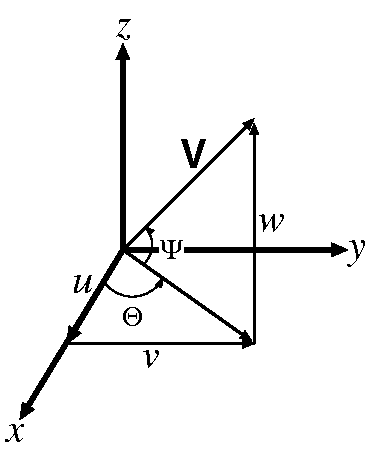
\includegraphics[width=5cm]{Figures/polar}
\caption{Definition of the polar angles used to specify the velocity components.}
\label{polar}
\end{center}
\end{figure}



\subsubsection{ Notes on Inflow Velocity Specifications}

A typical inflow boundary might be specified as:
\begin{verbatim}
  inflow(p=5000.0 psi,T=273 K,u=100, normal)
\end{verbatim}
but there are also two possible specifications for rotating flows: rigid body rotation
(helical flows) and a fixed swirling flow angle.  Rigid body rotation
is specified using the {\tt rotAxis}, {\tt rotCenter}, and {\tt
rotSpeed} boundary condition options, where {\tt rotAxis} is a vector
that defines the axis of rotation, {\tt rotCenter} is a point on the
rotation axis, and {\tt rotSpeed} is the rotational speed given by
default in revolutions per minute (rpm).  The rotation is defined by the
right-hand rule, thus a positive rotation speed about the $x$-axis {\tt
rotAxis} will produce positive $z$ components of velocity when the value
of $y$ is positive.

Alternatively, it is possible to specify a fixed swirl angle whereby
the direction of the velocity will rotate about a center axis.  This
is done using the specification of {\tt swirlAxis}, {\tt
swirlCenter}, and {\tt swirlAngle}.  The specification is similar to
the rotating flow specification, with the specified rotating flow
conforming to a right-handed coordinate system.

Both rigid body rotation and swirling flows can be specified for any
inflow boundary condition ({\tt inflow}, {\tt supersonicInflow}, {\tt farfield}, {\tt fixedMass},
and {\tt isentropicInflow}).  When these conditions are specified, the
direction of the velocity vector is modified to conform to the
rotating conditions, but the magnitude of the velocity is preserved.
For {\tt fixedMass} and {\tt isentropicInflow}, best results
will be achieved if the boundary surface is planar and normal to the
axis of rotation.  The following are some examples:

\begin{verbatim}
  inflow(p=5000.0 psi, T=274 K, u=100 m/s, 
         swirlAxis=[1,0,0], swirlCenter=[-1,0,0], swirlAngle=5deg),
  fixedMass(mdot=1kg/s, T0=300K, 
            rotAxis=[0,1,0], rotCenter=[0,0,0], 
            rotSpeed=3000 rotations/minute),
\end{verbatim}

\subsubsection{ Notes on Setting Viscous Boundary Velocity }

A tangential velocity can be specified on viscous wall boundaries for
simulating wall translation and rotation.  To specify the translational
velocity, use the {\tt Uwall} parameter.  A rotating viscous wall is
specified using the {\tt rotAxis}, {\tt rotCenter}, and {\tt rotSpeed}
options, similar to rotating inflows.  A moving wall velocity
can be specified for either viscousWall or wallLaw boundary
conditions.  In addition, only the tangential part of the specified
velocity is used in the viscous velocity specification.  

{\center \it Examples}

A moving lid with a constant linear velocity is specified as:
\begin{verbatim}
  wallLaw(adiabatic, Uwall=[1,0,0]), // Wall moving at 1 m/s to right
\end{verbatim}
A rotating wall can be specified as:
\begin{verbatim}
  viscousWall(Twall=300K, rotSpeed=100 rpm, 
              rotAxis=[0,0,1], rotCenter=0),
\end{verbatim}
where the rotation axis is the $z$ axis.


\subsubsection{Integrated Forces and Moments}
\label{integrated_fm}

{\em FlowPsi} provides the integrated forces and moments about a moment
reference center specified by the user (the default moment center is
the origin of the coordinate axes).  The output for specific BCs as
well as all of the viscous walls is placed in the standard output as
well as in special files located in the \verb!/output! directory.  The
output file naming convention and the file format are discussed below.

The user specifies a moment reference center in the \verb!.vars! file for each BC over which integrated forces and moments are required.  For example,
\begin{verbatim}
  BC_4 = viscousWall(adiabatic, momentCenter = [1., 0.5, 0.])
\end{verbatim}
locates the moment reference center for \verb!BC_4! at \verb!(1.,0.5,0.)! meters (the default units are meters).

Both the inviscid pressure and viscous shear stresses are integrated
over each BC.  For axisymmetric flows in which a 2D grid is translated
in the $z$ direction\footnote{see the {\tt gridCoordinates} input
  option for further information on computing axisymmetric flows with
  2D translated grids.}, the integration is over the 3D surface area
resulting from a 360$^o$ rotation about the $x$-axis, and the
integrations over the boundary area are computed accordingly.  For the
BCs on which a \verb!momentCenter! is specified, {\em FlowPsi} also
computes the moments for each of these force contributions.  The
forces and moments are resolved into the three coordinate directions
($x,y,z$).  Note that for the inviscid pressure contribution, the
force actually integrated is ({\it{$p - p_{ref}$}}), where $p_{ref}$
is the user input gauge pressure ({\tt .vars} file input {\tt p0})
(default $p_{ref}$ = 0).

The integrated fluxes for a specific boundary are placed in a file named \verb!/output/flux_BC4.dat!, for example.  The output format in this file is:
\begin{verbatim}
iteration, simulation time, mass flux, Fx, Fy, Fz, energy flux, area
\end{verbatim}
where \verb!Fx, Fy, Fz! are the total momentum fluxes (viscous plus inviscid) in each coordinate direction.  Similarly, the moments are placed in a file named \verb!/output/moment_BC4.dat!, and the file format is:
\begin{verbatim}
iteration, simulation time, Mx, My, Mz, RefMx, RefMy, RefMz
\end{verbatim}
where \verb!Mx, My, Mz! are the actual moments ($N$-$m$) relative to the defined \verb!momentCenter!, and \verb!RefMx, RefMy, RefMz! are the reference moments based on the integration of ({\it{$p - p_{ref}$}}) about the \verb!momentCenter!.

The force integrations over each BC surface are defined as follows:

\begin{equation}
F_x = \int{d\textbf{F} \cdot n_x dA}
\end{equation}

\begin{equation}
F_y = \int{d\textbf{F} \cdot n_y dA}
\end{equation}

\begin{equation}
F_z = \int{d\textbf{F} \cdot n_z dA},
\end{equation}
where $d\textbf{F}$ is the sum of the viscous and inviscid momentum fluxes on a surface with area $dA$, and ($n_x,n_y,n_z$) are the components of the surface normal vector.  The moment integrations are:
\begin{equation}
\textbf{M} = - \int{ \bf{(r - r_0)} \times \textbf{F} \textit{dA}} ~ ,
\end{equation}
where $\bf{r_0}$ is the user specified \verb!momentCenter! vector, and
$\bf{r}$ is the face center location of $dA$.  The {\em flowPsi}
output contains the ($x,y,z$) components of the total moment vector
$\textbf{M}$.  For axisymmetric flows in which the 2D grid is
translated in the $z$ direction, $F_x$ and $F_y$ take on the
integrated value while $F_z = 0$.  Similarly, $M_x = M_y = 0$, and
$M_z$ takes the integrated value.  Note that the moment integration is
consistent with the aerodynamic convention for pitch, roll, and yaw
({\it{i.e.}}, positive moments occur for pitch up, roll to the right,
and yaw to the right when viewed from the pilot's perspective).

%% \subsubsection{ Notes on Boundary Surface Integrations}

%% The code outputs integrated momentum, mass, and energy fluxes across
%% each boundary.  In addition an integrated moment of any given boundary
%% condition can be provided by specifying the momentCenter in the
%% specific boundary condition.  For example:

%% \begin{verbatim}
%%     BC_1=viscousWall(adiabatic,momentCenter=[0,0,0])
%% \end{verbatim}

\section{Relative Motion Problems using {\em FlowPsi}}

{\em FlowPsi} can be used to simulate moving bodies using an unstructured
over-set technique.  The over-set technique can be used with or without
hole-cutting.  Usually for relative motion in turbo-machinery
applications, hole cutting can be avoided through careful design of
the mesh components.  The most important tool in developing
simulations with relative motion is the interface boundary condition.
This boundary condition is applied at the boundary faces that are at
the edge of two grid regions.  Values are interpolated automatically
from neighboring meshes at the interface boundary condition.
Generally this boundary condition can be used for either overlapping
meshes or meshes that just slide along a common surface (but are not
point matched).

In order to move components independently, one must first create a grid
that contains volume tags that identify the meshes associated with
each component.  Each component mesh is generated
separately, and then all of the meshes are merged using the {\tt
  vogmerge} utility.  During the merging step, one provides
volume tags associated with each component grid.  For example, to merge the
rotor and stator components into a single grid from two grids called
'rotor.vog' and 'stator.vog', one would execute the following command:
\begin{verbatim}
vogmerge -g rotor.vog -tag Rotor -g stator.vog -tag Stator -o pump.vog
\end{verbatim}
This command combines the two grids for the rotor and stator into a
single grid called 'pump.vog'.  The cells of the pump grid that come from
{\tt rotor.vog} are tagged with ``Rotor'', and the cells of the pump grid
that come from {\tt stator.vog} are tagged with ``Stator''. 

Once a grid with the appropriate embedded volume tags and interface
boundary surfaces are defined, it is possible to move each component
independently using the {\tt componentMotion} variable in the {\tt vars}
file.  If this variable is defined, then the motion of each component will be specified by the user (note that if no componentMotion variable exists, then one can still use the overset boundary conditions, but all of the mesh components will remain stationary.).  There are several options for component motion:
\begin{enumerate}
\item {\tt stationary} 

Use this option to indicate that a given component does not move in
the simulation.
\item {\tt rotation}

This option is used to define the fixed rotation rate of the component.
The arguments to this option are {\tt axis},
which specifies the axis of rotation, {\tt center}, which specifies a
point on the rotation axis, and {\tt speed}, the rotation rate in
revolutions per minute (rpm).

\item {\tt prescribed}

This option is used to specify that the component motion is
given by a user defined data file.  This selection has no
arguments.  The file name is derived from the component tag name,
and the naming convention is {\tt motion\_TAG.vog}, where {\tt TAG} is
the tag name given to the component in the {\tt
  vogmerge} step.  The file starts with an integer number that specifies
the number of data entries in the file.
The data entries in the prescribed motion file (one entry per line) then
consist of time in seconds, followed by the three coordinate
positions of the center of mass in meters, followed by the four
components of a quaternion that describes rotations about the center
of mass.  Interpolation between the given data is accomplished using a cubic
spline.  In order to specify derivative discontinuities in the data,
repeat a data entry twice.

\end{enumerate}

\subsection{Specifying motion in a relative frame}

In some cases, one will specify the motion of a component relative to
another component's reference frame.  For example, one may describe the
rotation of the propellers of an airplane relative to the airplane's
coordinates.  If the airplane follows a prescribed motion, it is
naturally expected that the propellers will follow the same prescribed
motion.  In order to specify that the above motion is described in a
relative frame, one uses {\tt componentHierarchy} to define the
parent child relationship between objects.  If there is no motion
prescribed in a frame relative to another, then this option is not
needed.  Details on the usage of {\tt componentHierarchy} are given in
Section \ref{prob_description_file}.

\subsection{Hole Cutting}

When motion can be prescribed such that it occurs along sliding,
non-matched surfaces or along overlapping interface boundary
conditions that do not intersect other boundary faces, then hole
cutting can be avoided.  This reduces the number of cells needed and
improves run times.  However, it is impossible to describe more
general motion, such as two bodies that come in close proximity,
without hole cutting.  To employ hole cutting, a grid is first created
around an object that will be moving in the domain.  Usually the outer
envelope of this grid (where the interface BC is applied) will be a
simple geometric shape such as a sphere, cylinder, or body of
revolution.  Hole cutting is enabled by adding a definition for {\tt
  componentGeometry} to the {\tt .vars} file. (Note: adding {\tt
  componentGeometry} to the {\tt .vars} file enables the hole cutting
feature.).  In the component geometry input, the geometry of the outer
envelope of given mesh components will be specified.  At least one of
the mesh components will not be given any geometry description as this
mesh will serve as the background mesh.

When employing hole cutting, one does not need to be concerned
with the overlap of the outer interface boundary of a component since
the hole cutting will automatically cut cells according to the
distance of the cell to surfaces from other tagged regions.  Thus
when the interface surface overlaps geometry from another grid, the
grids will be cut along the surface of equal distance between the two
component surfaces.


\section{{\em FlowPsi} Pre- and Post-processing Utilities}

\subsection{{\em FlowPsi} Pre-processing Utilities}

\subsubsection{\tt ugrid2vog}

This converter allows one to convert {\it SolidMesh} or {\tt aflr3}
mesh files to the volume grid representation used by {\em FlowPsi}.  This
command can be run in parallel using mpirun for faster processing of
large meshes.  By default, the command will detect if the input file is
binary or ASCII, but you can force it to read a binary {\tt .b8.ugrid}
file using the {\tt -b} option.  The converter also has a {\tt -o}
option to disable optimizations that would change the numbering of
nodes and cells in the mesh from the given {\tt ugrid} file.
Generally this option would only be used if it is important for the
grid conversion to preserve the original node ordering.  Additionally,
you may input the units of the ugrid mesh (default is meters) with the option {\tt -in}
for inches, {\tt -ft} for feet, {\tt -cm} for centimeters, or {\tt -mm} for millimeters.  If another
unit is needed, you may use the {\tt -Lref} option. For example, if the
input grid named {\tt "wingsection.b8.ugrid"} is
non-dimensionalized with respect to a reference length
of 1.57 inches, you would use the command:
\begin{verbatim}
ugrid2vog -Lref "1.57 inch" wingsection
\end{verbatim}

\subsubsection{\tt xdr2vog}

This converter allows one to convert the older XDR format mesh files
to the volume grid representation used by {\em FlowPsi}.  This command can be
run in parallel using mpirun for faster processing of large meshes.
The converter has a {\tt -o} option to disable optimizations that
would change the numbering of nodes and cells in the mesh from the
given XDR mesh file.  Additionally, you may input the units of the XDR
mesh with the option {\tt -in} for inches, {\tt -ft} for feet, {\tt
  -cm} for centimeters, or {\tt -mm} for millimeters.  With no option,
{\tt xdr2vog} will assume the input is in meters.  The {\tt -Lref}
option can be used as with {\tt ugrid2vog} to specify other unit
systems.  

\subsubsection{\tt vogmerge}

The {\tt vogmerge} utility allows one to combine VOG file grids, apply
geometric transformations to the grids, rename boundary tags, and
apply volume tags.  Use options 

\begin{verbatim}
vogmerge -g input.vog -zscale -1 -g input.vog -o combine.vog
\end{verbatim}

Note that the geometric transform options are applied to the grid of
the preceding {\tt -g} options.  If many geometric transforms are
specified, then they are applied in the given order.  Finally, for
each grid, one may apply a volume tag using the {\tt -tag} option.
This is used when creating grids for simulations using relative
motion.  For example, to perform a simulation on turbo-machinery that
included a rotor and stator section, one would generate two grids, one
for each component, and then merge them using the following vogmerge
command:
\begin{verbatim}
vogmerge -g rotor.vog -tag rotor -g stator.vog -tag stator -o turbo.vog
\end{verbatim}
Once can then prescribe different motions to each grid using the {\tt
  componentMotion} variable in the {\tt .vars} file using the volume tags
{\tt rotor} and {\tt stator}.

Executing {\tt vogmerge} without any options will provide a usage guide.
The current options to {\tt vogmerge} are:

\begin{table}[htbp]
\begin{center}
\begin{tabular} {|l|l|}
\hline
option & description\\
\hline\hline
  {\tt -g} {\it gridfile}           & Specify input grid filename \\
  {\tt -o} {\it gridfile}           & Specify output grid filename \\
  {\tt -xshift} {\it value}         & translate grid in x-coordinate\\
  {\tt -yshift} {\it value}         & translate grid in y-coordinate\\
  {\tt -zshift} {\it value}         & translate grid in z-coordinate\\
  {\tt -xscale} {\it value}         & scale grid in x-coordinate\\
  {\tt -yscale} {\it value}         & scale grid in y-coordinate\\
  {\tt -zscale} {\it value}         & scale grid in z-coordinate\\
  {\tt -scale}  {\it value}         & scale grid in all coordinates\\
  {\tt -xrotate} {\it value}        & rotate about x-axis (degrees)\\
  {\tt -yrotate} {\it value}        & rotate about y-axis (degrees)\\
  {\tt -zrotate} {\it value}        & rotate about z-axis (degrees)\\
  {\tt -bc} {\it oldname}{\tt ,}{\it newname} & rename boundary surface\\
  {\tt -glue} {\it bcname}          & glue this boundary to a matching bc\\
  {\tt -tag} {\it name}             & specify volume tag for input grid\\
\hline
\end{tabular}
\end{center}
\end{table}

\subsubsection{\tt cobalt2vog}

The {\tt cobalt2vog} grid converter will convert an ASCII unformatted {\it Cobalt 60} grid format file and convert it into a VOG grid suitable for use with {\em FlowPsi}.  The extension on the cobalt grid should be {\tt cog}.

\subsubsection{\tt plot3d2vog}

The {\tt plot3d2vog} grid converter will convert multi-block plot3d
files into an VOG file format compatible with {\em FlowPsi}.

\subsubsection{\tt fluent2vog}

The {\tt fluent2vog} grid converter will convert fluent {\tt .msh}
files to the VOG file format for use with {\em FlowPsi}.

\subsubsection{\tt ccm2vog}

The {\tt ccm2vog} grid converter will convert Star CCM+ grids to the VOG file format for use with {\em FlowPsi}.


\subsubsection{\tt vogcheck}

The {\tt vogcheck} utility is a grid quality assessment tool for {\em FlowPsi}.
This program can be run in parallel for larger grids using mpirun.
The program outputs an overall assessment of the grid quality in the
range of {\tt UNUSABLE}, {\tt marginal}, {\tt poor}, {\tt good}, and {\tt
  excellent}.  A grid that is identified as {\tt UNUSABLE} will
probably not be useful for {\em FlowPsi} simulations.  Grids marked as {\tt
  marginal} may provide numerical robustness problems for {\em FlowPsi}.  It is
suggested that the user query the cause of poor mesh quality for these
grids.  Grids identified as {\tt poor} may be acceptable for
running with {\em FlowPsi}, but accuracy will probably be degraded in some
regions.  Any grid marked as {\tt good} or {\tt excellent} has a mesh
quality that is suitable for high quality solutions using {\em FlowPsi}.

To query the mesh quality, one can extract the mesh quality measures
from {\tt vogcheck} from iteration {\tt 0}.


\subsection{{\em FlowPsi} Post-processing utilities}

\subsubsection{Probe Output}

The {\em FlowPsi} code can output variables at a specified location to a file every
iteration using probes.  There is no limit to the number of probes allowed.
The specification in the {\tt .vars} file is:
\begin{verbatim}
probe: <probe1=[0,0,0],probe2=[1,0,1]>
\end{verbatim}
where the units of the point are in meters if units are not explicitly
specified with the point locations.  Probes will generate output files
in the form {\tt probeX.dat}, where {\tt X} is the probe number.
The file contains lines with the following information:
\begin{verbatim}
  <ncycle> <stime> <T> <p> <rho> <a> [ <U> ] [ <pos> ] <dist> <mass fractions>
\end{verbatim}
where:
\begin{verbatim}
  <ncycle> is the iteration number of the simulation
  <stime> is the simulation time
  <T> is the temperature
  <p> is the pressure
  <rho> is the density
  <a> is the sound speed
  <U> is the velocity vector
  <pos> is the position of the probe
  <dist> is the distance between the probed value and the position given in the
         input file.
\end{verbatim}

\subsubsection{Plot Format Converter}
\label{sec:converter}
See the {\tt plot\_freq} item for an explanation of how to generate data
for visualization in the {\tt output} directory.  These files are annotated by the
iteration number (modulo the {\tt plot\_modulo} value).  Once generated, the
{\tt extract} program can be used to generate various plot files for post
processing programs such as {\it FieldView},{\it EnSight}, {\it
TecPlot}, and {\it 2dgv}.  The first argument to {\tt extract} specifies
which post processing software format to use.
Table \ref{tab:extractpost} gives a list of the
currently supported post processing selectors for {\tt extract}.  Other
options may follow that are specific to the particular post processor.
The user then provides the problem name (this is the name of the {\em FlowPsi}
{\tt .vars} file without the {\tt .vars} extension),
the iteration number to extract from, and
a list of variables to extract.  The default variables output by {\em FlowPsi}
are given in table \ref{tab:extract}.  The 2dgv post processing
package will only allow the specification of a single variable, while
all others support visualization of multiple scalar and vector values.
The form of an extract command is:

\begin{verbatim}
extract -<package> [options] <problem name> <time step> <variable(s)>
\end{verbatim}

Note that documentation of how to use {\tt extract} can also be obtained by
executing the command {\tt extract} without any arguments.


\begin{table}[htbp]
  \begin{center}
    \leavevmode
    \begin{tabular}{|l|l|}
      \hline
      post-processor option & purpose \\
      \hline
      {\tt -fv} & {\it FieldView} postprocessing\\
      {\tt -en} & {\it EnSight} postprocessing\\
      {\tt -tec} & {\it TecPlot} postprocessing\\
      {\tt -2d} & {\it 2dgv} postprocessing\\
      {\tt -cut} & Dump a cutting plane for {\it 2dgv} postprocessing\\
      {\tt -ascii} & Dump selected nodal data to an ASCII file\\
      {\tt -mean} & Generate mean and variance from family of variables\\
      {\tt -surf} & Extract boundary surface mesh\\
      \hline
    \end{tabular}
    
    \caption{extract post-processor selectors}
    \label{tab:extractpost}
  \end{center}
\end{table}

\begin{table}[htbp]
  \begin{center}
    \leavevmode
    \begin{tabular}{|l|l|}
      \hline
      Key & function \\
      \hline
      r & density \\
      p & $log_{10}$(pressure) \\
      P & actual pressure in SI units \\
      u & fluid speed \\
      0, 1, 2 & Cartesian components of fluid velocity \\
      v & velocity vector \\
      m & Mach number \\
      t & temperature \\
      a & sound speed \\
      tau & wall shear stress (vector) \\
      taumag & wall shear stress magnitude (scalar)\\
      qdot & wall heat flux \\
      tw & wall temperature \\
      pw & wall pressure \\
      bt & boundary temperature \\
      bpg & boundary gage pressure \\
      br & boundary density \\
      mdot & boundary mass flux \\
      \hline
    \end{tabular}
    
    \caption{{\tt extract} command keys}
    \label{tab:extract}
  \end{center}
\end{table}

The {\em FlowPsi} code will optionally output other scalar and vector data
when these variables are provided in the {\tt plot\_output} list
in the {\tt .vars} file.  
%%The scalar variables that can be optionally written
%%by {\em FlowPsi} are given in Table \ref{tab:nodalextract}, and the vector
%%variables are given in Table \ref{tab:vectorextract}.  
For example, to
extract the turbulence model scalars {\tt k}, {\tt w}, and {\tt tmu},
one would place the following in the {\tt .vars} file:
\begin{verbatim}
// Note, no spaces between variables, just commas
plot_output: k,w,tmu
\end{verbatim}

Now the variables can be extracted for visualization with {\it FieldView} for the case {\tt plume} at iteration {\tt 100} using the command:
\begin{verbatim}
extract -fv plume 100 k w tmu
\end{verbatim}


\subsection{Surface Data Output Options}

By default {\em FlowPsi} outputs data for volume nodal data and surface facet
information.  For very large meshes or time accurate simulations where
frequent output is required, the size of the volume data can become
prohibitive.  To facilitate more control over the amount of output
data {\em FlowPsi} produces, users can instead choose to write out surface data
for a specific subset of surfaces, variables, and times.  By default
individual surface data is not written out, but the output for any
boundary surface can be enabled by adding the variable {\tt plotFreq}
and {\tt plotVars}.  The variable {\tt plotFreq} tells the frequency
of plotting for that boundary surfaces whereas {\tt plotVars} is set
set to a list of variables that will be output for that boundary
surface.  For example, if one wanted to output surface pressures and
temperatures every 10 cycles for a viscous wall boundary one could
enter in the {\tt boundary\_conditions} line:
\begin{verbatim}
bladerow = viscousWall(adiabatic, plotFreq=10, plotVars=[pg,t]),
\end{verbatim}

In addition to boundary surface data, {\em FlowPsi} can also output clip
surfaces in the form of clip planes or isosurfaces.  The clip surface
capability is enabled by adding the variables {\tt clipFreq} and {\tt
  clipSurfaces} to the vars file.  The {\tt clipFreq} variable provides an
integer which will be the frequency of clip surface output, while the
{\tt clipSurfaces} gives a list of surface names with clipping
specifications.  The clipping specification can either be a {\tt
  plane} or an {\tt isosurface}.  For a clip plane the specification
requires a {\tt point} on the plane and the {\tt normal} vector of the
plane.  The iso-surfaces specifications gives a variable assignment
where the iso-surface will be computed.  An example of clip surfaces
is given in the specification:

\begin{verbatim}
clipFreq: 25
clipSurfaces: < zcut10 = plane(point=[0,0,10],normal=[0,0,1]),
                t1000  = isosurface(t=1000),
                t0500  = isosurface(t=500)>
\end{verbatim}

The previous example will generate cut surfaces every 25 timesteps
where the cut surfaces include the surface named ``zcut10'' which is
the plane formed by $z=10$, the ``t1000'' isosurface where temperature
is 1000 Kelvin and the ``t500'' isosurface where temperature is 500
Kelvin.  Note, the input for the isosurface command cannot accept unit
specification and instead will always be interpreted in terms of
{\em FlowPsi}'s output default which is the MKS unit system.  Also note, any
variable that was specified for plotting on the volume mesh (those
listed in {\tt plot\_output} or {\tt plot\_output\_exclusive} will be
written out for these surfaces.

\subsection{Mean and Variance Output}

For hybrid RANS/LES or DES simulations, it is useful to compute mean
and variances of output variables.  There are two methods provided to
allow users to extract this type of information from a simulation:
offline and online.  The offline approach is implemented as part of
the {\tt extract} utility with the {\tt -mean} option.  The extract
utility can read in a sequence of output scalars or vectors that were
written out by {\em FlowPsi} and compute mean and variance values
which are then written back out to the output directory.  The {\tt
  extract} utility can then be used to visualize the resulting mean
and variance values.  To extract these values, use the argument {\tt
  -mean} followed by {\tt -end} with the ending iteration and {\tt
  -inc} with the iteration increment.  Extract starts with the usual
given extract iteration number and averages consecutive plot files at
the provided increment until the ending iteration is reached.  The
mean values are then written to the output directory as the variable
with {\tt Mean} appended for the mean and {\tt Var} for the variance.
For vector valued variables, the covariance is also output as {\tt
  Cuv}, {\tt Cuw}, and {\tt Cvw} for the covariance of the {\it x-y},
{\it x-z}, and {\it y-z} components, respectively.  These variables
can then be extracted in the usual way for visualization.

The online method for mean and variances is enabled by adding the
following line to the top of your {\tt .vars} file (before the first brace, \{ ):

\begin{verbatim}
loadModule: onlineStats
\end{verbatim}

In the {\tt .vars} file, you will also need to add a definition for
the averaging window size using the {\tt meanFreq} variable.  The
average will automatically reset when the window size is reached.
Alternatively, the code can perform exponential averaging if the
variable {\tt useExponentialMean} is set to {\tt on}.  In the
exponential averaging approach, the averaging weight is computed based
on the window provided by {\tt meanFreq}.  When online averaging is
enabled, the code will output the variables listed in table
\ref{tab:onlinestats}.  Note that these variance values are the square
of the RMS value.  Also not that the velocity mean and variances are
Favre averaged while

\begin{table}[htbp]
  \begin{center}
    
    \leavevmode
    \begin{tabular}{|l|l|}
      \hline
      Key & function \\
      \hline
      {\tt tmean} & average temperature \\
      {\tt tvar} & variance in temperature \\
      {\tt pgmean} & mean gage pressure \\
      {\tt pgvar} & variance in gage pressure\\
      {\tt rmean} & mean density\\
      {\tt umean} & Favre mean velocity vector\\
      {\tt uvar} & Favre variance in velocity components\\
      {\tt ucovar} & Favre covariance of velocity components\\
      \hline
    \end{tabular}
    
    \caption{variables output by the {\tt onlineStats} module}
    \label{tab:onlinestats}
  \end{center}
\end{table}
\subsection{The Grid Motion Module}

The grid  motion module  smoothly projects deformations  from surfaces
into the  volume mesh.  The algorithm  used by the  grid motion module
employs  an algebraic interpolation  method that  is fast  and robust.
High speed is  obtained through a tree code  acceleration which allows
the interpolation to be evaluated to within a specified accuracy.


\subsubsection{Theoretical Background}
The deformation of the volume mesh can be viewed as a projection of
deformations and rotations from the surface into the volume.  For
general mesh deformations the local surface rotations can estimated
once the displacements are given for each node of the surface mesh.
In the algorithm described in this paper we estimate local rotations
by finding the closest rotation about the node that best matches the
relative displacements of all edges and normals from surface facets
that reference the given node.  Using this information, the
displacement field presented by any surface node can be described as a
rigid body motion.  In our approach, the global deformation field is
given as a weighted sum of these nodal rigid body displacements, where
node $i$ on the deforming surface presents a displacement field,
denoted $\vec{s}_i(\vec{r})$, that is written as
\begin{equation}
\vec{s}_i(\vec{r}) = M_i \vec{r} + \vec{b}_i - \vec{r}, 
\end{equation}
where $M_i$ is a rotation matrix, $\vec{b}_i$ is a displacement
vector associated with the $i^{th}$ node, and $\vec{r}$ is a coordinate
vector in the original mesh.  The displacement field in the volume
mesh is then described through a weighted average of all boundary node
displacement fields as given by
\begin{equation}
\vec{s}(\vec{r}) =\frac{ \sum w_i(\vec{r}) \vec{s}_i(\vec{r})}
    { \sum w_i(\vec{r})}.
\label{eq:deformation}
\end{equation}

For the interpolation weight function, we choose a weighting that is a
function of the reciprocal of distance.  We utilize a two-exponent
form of the weighting function so that we can preserve near-boundary
deformations while providing a smooth transition in the interpolation
to blend deformations in the bulk of the volume mesh.  We also use the
area of the surface facet in the weighting function so that mesh
refinement of a region does not increase its influence in the
interpolation method.  The resulting weighting function is given as
\begin{equation}
w_i(\vec{r}) = A_i * \left[
  \left(\frac{L_{def}}{||\vec{r}-\vec{r}_i||}\right)^a +
  \left(\frac{\alpha L_{def}}{||\vec{r}-\vec{r}_i||}\right)^b \right],
\label{eq:weight}
\end{equation}
where $\vec{r_i}$ is the position of point $i$, $A_i$ is the area
weight assigned to node $i$, $L_{def}$ is an estimated length of the
deformation region, $\alpha$ is an estimated size of the near body
influence region expressed as a fraction of $L_{def}$, and $a$ and $b$
are user-defined exponents.  Numerical experimentation suggests that
$a=3$ and $b=5$ provide the best-quality results.  The $L_{def}$
parameter may be specified by the user, but it is usually determined
automatically by computing the maximum distance any mesh node is from
the mesh centroid.  The alpha parameter controls how much weight is
given to deformations of nearby surfaces relative to more distant
ones.  Generally, this will need to be increased with the variability
in surface displacements.  This appropriate automatic determination of
$\alpha$ can be computed from the deviation of the boundary
displacement field from the mean boundary displacement given by
\begin{equation}
\vec{s}_{mean} = \sum_{i=1}^{N} a_i * \vec{s}_i(\vec{r}_i),
\end{equation}
where $a_i=A_i/\sum_{j=1}^N A_j$ is the normalized node weight and
 $\alpha$ is then determined through the following expression:
\begin{equation}
\alpha = \frac{\eta}{L_{def}}\max_{i=1}^N  ||\vec{s}_i(\vec{r}_i)-\vec{s}_{mean}||.
\label{eq:dynamicalpha}
\end{equation}
The $\eta$ term is a user defined parameter that expresses how far
into the domain a displacement should be ``absorbed.''  Numerical
experiments have found that a value of $\eta=5$ provides satisfactory
results in most cases.  Generally, we limit $\alpha$ to be $0.1$ or
greater to guarantee that a region of rigid deformation is maintained
in boundary layer regions to preserve viscous mesh quality.  This
defines our baseline direct interpolation algorithm.  Our numerical
experiments show that this approach is able to produce high-quality
meshes for large deformations and also is able to preserve mesh
orthogonality near the boundary surfaces.

\subsubsection{Optimizations}

For two-dimensional problems where the number of boundary nodes is
relatively small, the above algorithm runs quite fast.  However, for
three-dimensional problems, the surface nodes grow at a rate of
$O(n^\frac{2}{3})$, where $n$ is the total number of nodes in the
simulation.  Therefore, the cost of the above algorithm becomes
$O(n*n^\frac{2}{3})=O(n^\frac{5}{3})$.  Although the algorithm
parallelizes well, the cost of the deformation calculation quickly
becomes dominant for three-dimensional cases.  However, for mesh
deformation, the accuracy of this evaluation is not critical and only
needs to be accurate to a fairly large fraction of the mesh spacing.
Also, the form of the sum is similar in form to gravitational
potential equations that are solved for N-body simulations.  It is
therefore reasonable to look towards tree-code optimizations similar
to N-body algorithms such as Barnes-Hut\cite{Barnes.1986} and
FMM\cite{Greengard.1987}.  Using these approaches, the cost of the
deformation step could be reduced to $O(n \log n)$, or even $O(n)$ if
suitable kernels for the multipole and local expansions are found.

The Barnes-Hut tree-code algorithm requires that we have an
approximation for the influence of a set of points at some distance
and that we have an estimate for the error in the approximation.  In
the case of N-body simulations, potential theory can be used to
express the influences of a collection of bodies as a multipole
expansion about the centroid.  A truncated expansion can be used to
provide an approximation and also an estimate on error bounds.
Unfortunately, the sums given in equations (\ref{eq:deformation}) and
(\ref{eq:weight}) do not satisfy potential theory and so an analytical
approach to forming a multipole expansion is not readily available.

Lacking this infrastructure, we find an alternative way of
constructing a suitable approximation to the effects of a collection
of particles.  First, we focus on approximating the sum
\begin{equation}
f(\vec{r}) = \sum_{i=1}^N \frac{a_i}{||\vec{r}-\vec{r_i}||^3},
\label{eq:sum}
\end{equation}
where $a_i$ is the normalized node weight.  Instead of attempting to
find a multipole expansion for this sum, we instead focus on finding a
small set of pseudo nodes that can approximate the collection of
particles at a distance, essentially approximating a truncated
multipole expansion.  For example, to approximate a quadripole we
would use four points that share the same centroid as the collection
of points such that our sum is approximated by
\begin{equation}
f(\vec{r}) \approx \frac{1}{4}\left( \frac{1}{||\vec{r}-\vec{q}_1||^3}
+\frac{1}{||\vec{r}-\vec{q}_2||^3}
+\frac{1}{||\vec{r}-\vec{q}_3||^3}
+\frac{1}{||\vec{r}-\vec{q}_4||^3}\right),
\label{eq:approx}
\end{equation}
where $\vec{q}_1,\vec{q}_2,\vec{q}_3,$ and $\vec{q}_4$ represent the
locations of the four approximating pseudo nodes which we call
the quad-points or QPs.  Given the constraint that the QPs share the centroid of the collection given in equation \ref{eq:sum}, we can determine the location of $\vec{q}_4$ using the relation
\begin{equation}
\vec{q}_4 = 4~\left( \sum_{i=1}^N a_i \vec{r_i} \right) - \left( \vec{q}_1 + \vec{q}_2 + \vec{q}_3\right).
\label{eq:centroidconstraint}
\end{equation}

The three remaining QPs are found using a non-linear least squares that minimizes the error given by
\begin{equation}
err  =  ||f(\vec{r})-\frac{1}{4}\left( \frac{1}{||\vec{r}-\vec{q}_1||^3}
+\frac{1}{||\vec{r}-\vec{q}_2||^3}
+\frac{1}{||\vec{r}-\vec{q}_3||^3}
+\frac{1}{||\vec{r}-\vec{q}_4||^3}\right)||^2
\end{equation}
on the test sphere defined by $r=3R_e$ where $R_e$ is the radius of
the smallest centroid centered sphere that contains all of the points,
$\vec{r}_i$.  In our case we minimize the error at the 20 nodes of a
dodecahedron that is circumscribed by the test sphere.  We pick three
points arbitrarily from the collection of points to initialize the
non-linear least squares solve.  An example of this procedure is shown
in figure \ref{fig:QPs} where the small white points show a collection
of 128 random points sampled from the surface of one octant of the
unit sphere.  The dark gray inner region illustrates the enclosing
sphere with radius $R_e$, while the larger sphere illustrates the test
sphere where error is minimized.  The larger blue points show the
location of the computed QPs.  Once we have computed the QP locations,
we utilize 12 additional points on the sphere defined by the centroids
of the dodecahedron faces to sample the errors on the test sphere.
The errors in using the QPs to approximate the sum for both the third
and fifth powers are shown in table \ref{tab:error}.  The table shows
that the approximation error drops as a function of $1/r^2$ for
exponents three and five providing the needed model for approximation
errors.

\begin{figure}
  \begin{center}
    \noindent
    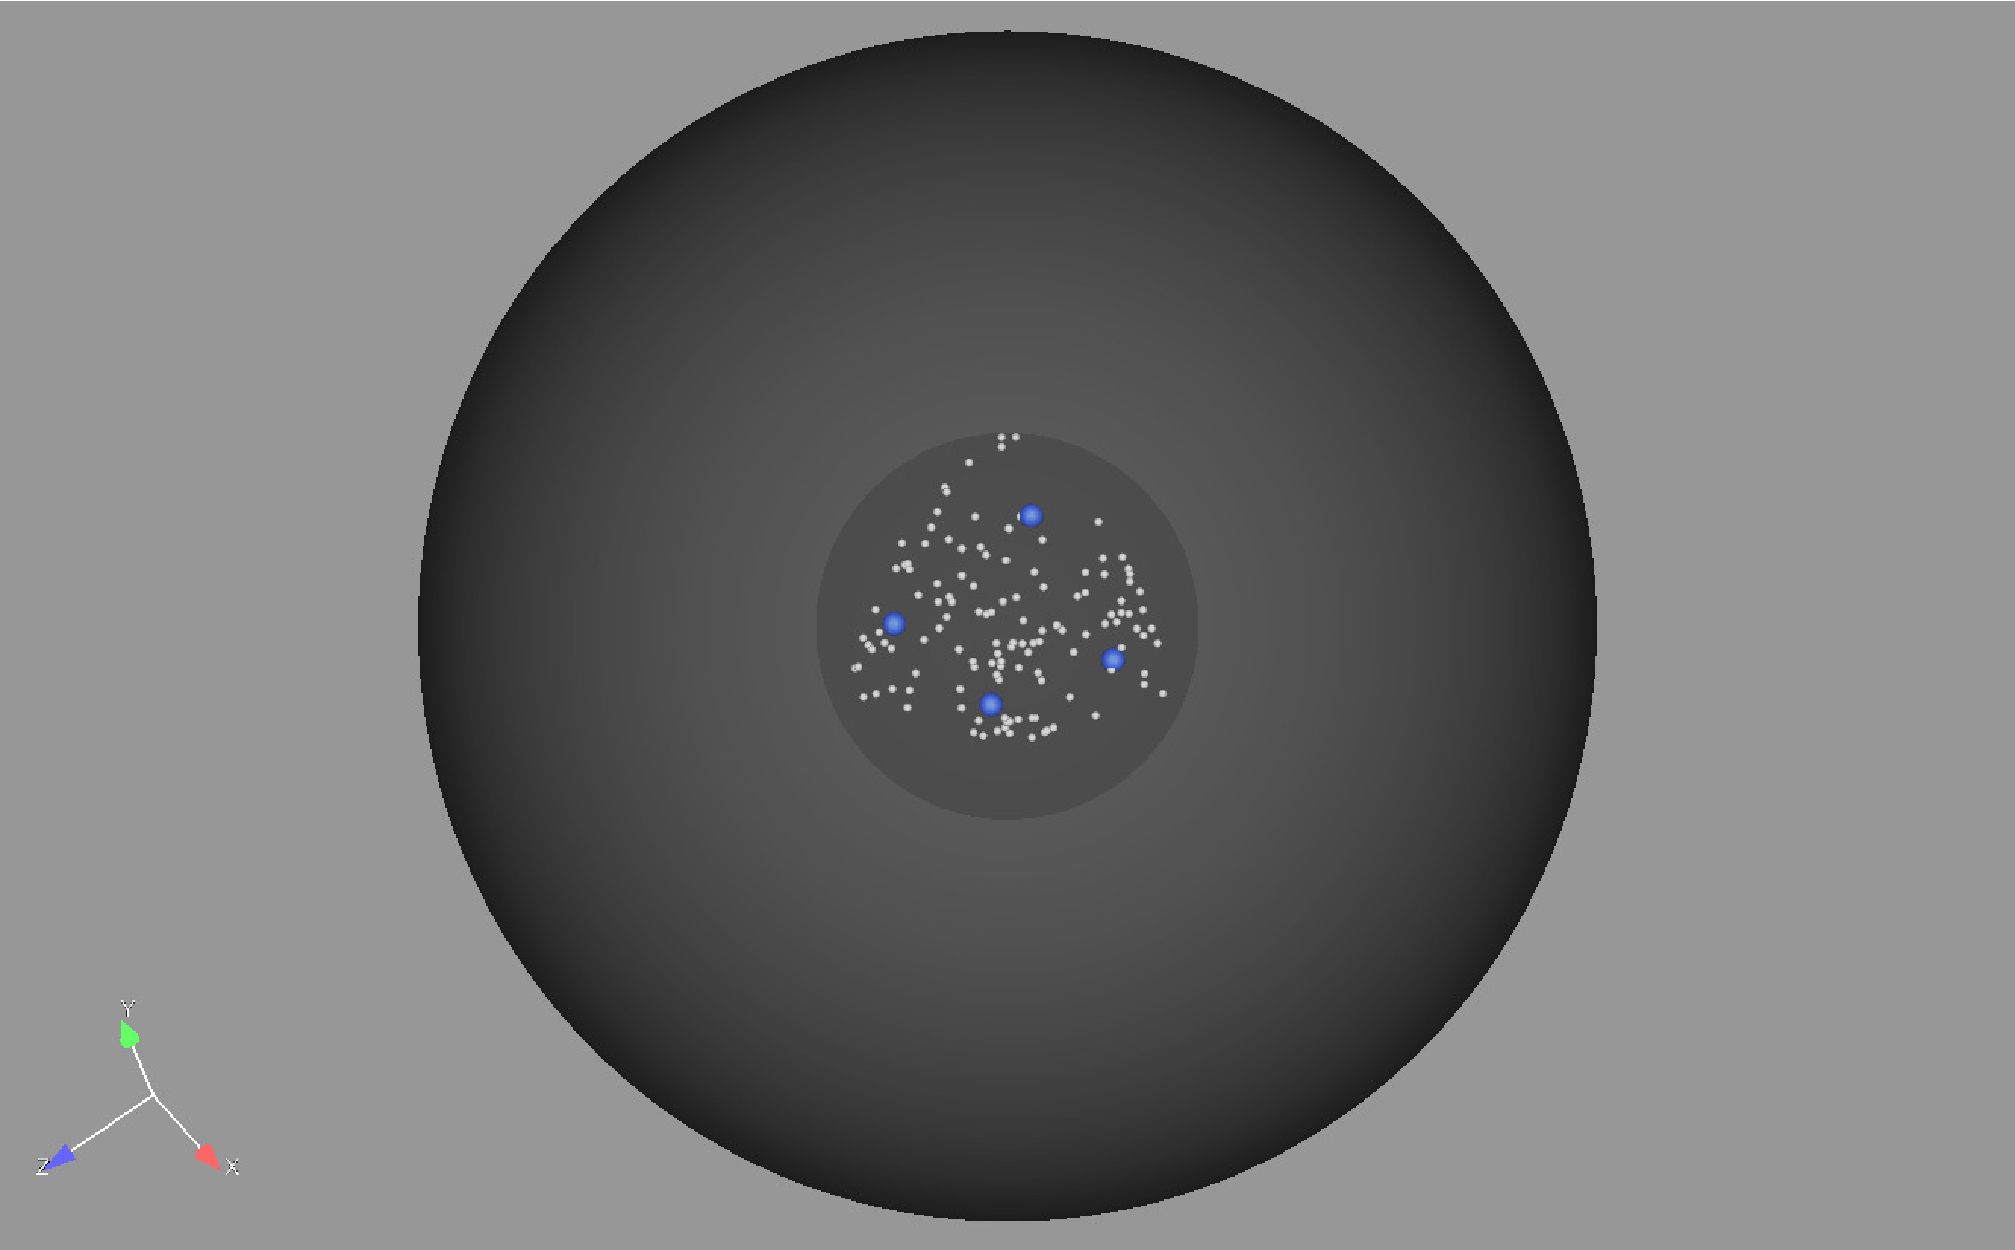
\includegraphics[width=0.75\textwidth]{Figures/points}
  \end{center}
  \protect\caption{Illustration of QP computation}
  \label{fig:QPs}
\end{figure}

\begin{table}[htbp]
\caption{Errors for QP approximation}
\label{tab:error}
\begin{center}
\begin{tabular}{|r||l|l|l|}
\hline
distance  & error         & error \\
(r)       & $(a_i/r_i^3)$  & $(a_i/r_i^5)$ \\
\hline\hline
$3 R_e$   & 0.967\%       & 3.34\%\\
$10 R_e$  & 0.0563\%      & 0.140\%\\
$20 R_e$  & 0.0124\%      & 0.0313\%\\
$40 R_e$  & 0.00290\%     & 0.00737\%\\
$80 R_e$  & 0.000717\%    & 0.00180\%\\
$160 R_e$ & 0.000184\%    & 0.000457\%\\
\hline
\end{tabular}
\end{center}
\end{table}

For general deformations, we also need to consider the implications of
the variation of the rotation matrices, $M_i$, and translation
vectors, $b_i$.  To approximate the effects of these terms, we use the
QPs found in the previous step, but perform a term-by-term least
squares fit in order to assign $M_i$ and $b_i$ to the four
approximation points, again preserving the centroidal value.  The
resulting approximations have similar accuracy profiles to those shown
in table \ref{tab:error}.

\begin{figure}
  \begin{center}
    \noindent
    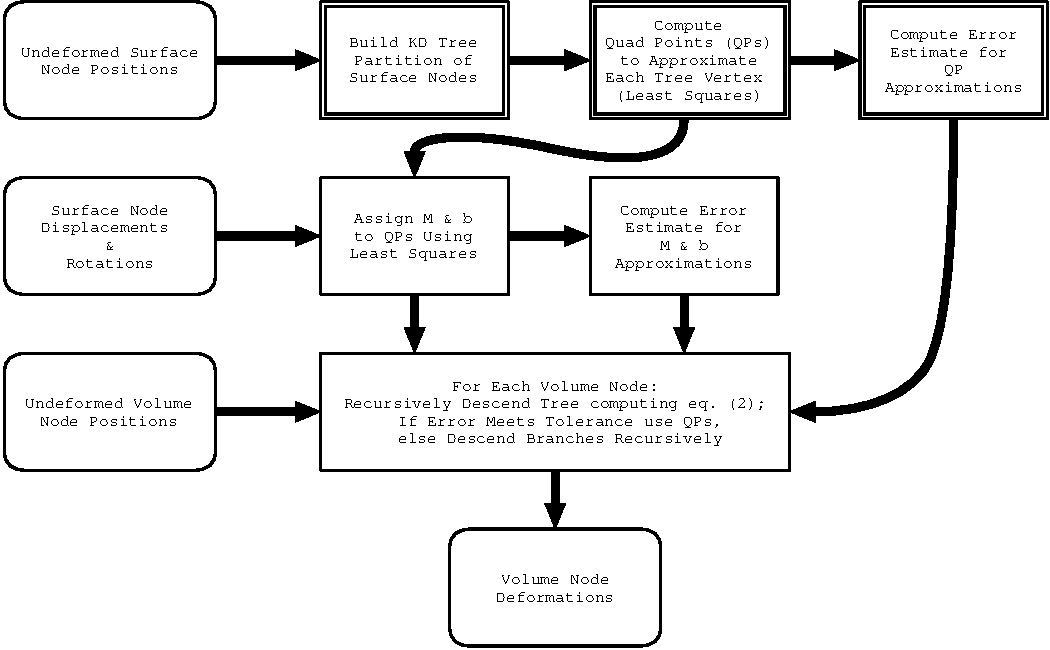
\includegraphics[width=0.75\textwidth]{Figures/fmdmflow}
  \end{center}
  \protect\caption{Mesh Deformation Software Architecture}
  \label{fig:architecture}
\end{figure}

From these approximations, we have the foundation to build a tree-code
fast evaluator.  The architecture of the tree-code mesh deformation
software is shown in figure \ref{fig:architecture}.  The boxes with
double lines only need to be evaluated once using the original
undeformed grids.  The remaining steps, because they depend on the
actual displacements, must be computed every time new displacements are
provided.  The first step is to build the KD-tree to spatially
partition the surface nodes.  To reduce the depth of the tree, we use
bins containing approximately 32 surface nodes for the leaves of the tree.
Once the spatial partition is established we then compute the QPs for
each vertex in the KD-tree.  Once the QPs are determined, the errors
at the test sphere can be measured.  The KD-tree vertices are then
populated with the centroid, containing sphere radius, and measured
errors.  

The final step in the deformation algorithm is evaluating deformations
for the mesh volume nodes (note the deforming surface nodes are
evaluated using the prescribed deformations).  The recursive evaluator
computes the numerator, denominator, and the error in the denominator
of equation (\ref{eq:deformation}).  If we are a leaf of the tree then
the deformation and weights are evaluated exactly forming the base
case of the recursive algorithm.  Otherwise we evaluate the error
associated with using the QP approximation at the current level.  If
the error bound is met, then return the approximate numerator and
denominator, otherwise sum the evaluation of the two children.  Note,
since we compute the accumulated error, there can be an advantage to
evaluating the parts of the tree that give larger weights as this
increases the error threshold for the remaining part of the tree.
Therefore we visit child vertices in the order of closest centroid
first to reduce computational cost.

The behavior of this algorithm automatically reduces errors near the
surface since in this region the nearby leaves will be evaluated as an
exact expansion.  Since the weights associated with these nearby
points will typically be much greater than more distant points, the
error in the boundary layer regions is generally very small regardless
of target error bound.  Further away from the surface we generally
only need the deformation error to be within small fraction of the
edge length.  Typically we find that this requirement is easily met
with a target relative error of just $1\%$.


\subsubsection{Grid Motion User Controls}

The grid motion module is activated by adding an appropriate
{\tt loadModule} command at the top of your vars file:
\begin{verbatim}
loadModule: gridMotion
\end{verbatim}

The global properties of the interpolation can be controlled by user
specified parameters.  In most cases these parameters will work very
well in their default setting, but in specific cases it may be helpful
to make changes.  These controls are represented by the following vars
file variables:

\begin{enumerate}
  \item {\tt gridMotionExpA}
    
    This is the $a$ coefficient described in the weight equation, eq. (\ref{eq:weight}).  This controls how deformations are blended away from the deforming surfaces.  The exponent is a positive integer with a default setting of 3.  A smaller setting will make the blending smoother with a greater risk of having grid line crossing, whereas a larger number will increase shearing in the mesh.  Generally it is good to leave this value as the default.
    
  \item {\tt gridMotionExpB}

    This is the $b$ coefficient described in the weight equation, eq.
    (\ref{eq:weight}).  This controls how deformations are blended for
    points close to the surface.  It is usually set to a larger value
    than $a$ so that the behavior near the body behaves in a more
    rigid manner preserving viscous mesh orthogonality.  The default
    setting for this is 5.

  \item {\tt gridMotionLref}
    
    This is the $L_{def}$ coefficient in the weight equation, eq.
    (\ref{eq:weight}).  This defines the average length over which the
    deformation will be distributed.  If this variable is not set,
    then the deformation length is computed by finding the most
    distant point in the mesh from the mesh centroid.  For many
    problems this is a good default value, but for specific cases,
    particularly where you know the deformation region is much smaller
    than the overall mesh, it may be helpful to set this value to
    something that is sensible to your specific mesh deformation case.

  \item {\tt gridMotionAlpha } 

    This is the $\alpha$ coefficient in the weight equation , eq.
    (\ref{eq:weight}).  This defines the fraction of the deformation
    length that will be reserved for more rigid near-body deformation.
    If this is not set then the value of $\alpha$ will be computed
    dynamically based on equation (\ref{eq:dynamicalpha}).  Usually
    the dynamic alpha provides better results than providing a
    constant value with this setting, so it is advised not to adjust
    this parameter.


  \item {\tt gridMotionAlphaFactor}

    This variable is the $\eta$ parameter in the dynamic alpha
    equation (\ref{eq:dynamicalpha}).  The dynamic alpha will increase
    the stiff region around bodies when they have more complex
    deformations.  The default value is set to 5 which appears to be
    sufficient for most applications.

  \item {\tt gridMotionAlphaFloor}

    This variable sets the minimum value for $\alpha$ that will be
    used when the dynamic alpha computation is being used.  This
    provides a guarantee that near wall regions will remain rigid and
    orthogonal.  The default setting for this value is 0.1.


  \item {\tt gridMoveErrorTol}

    This variable sets the error tolerance of the approximation
    algorithm.  It is a percentage of the minimum edge length attached
    to the node.  The default value is 0.1 which is usually sufficient
    for most applications.  A larger value will degrade mesh quality
    but may improve speed, while a smaller value can improve mesh
    quality if approximation errors were the cause.  Generally this
    value does not need to be changed from the default setting.

  \item {\tt gridDeformationSymmetry}

    This variable is set if you have a symmetry plane at $x=0$, $y=0$,
    or $z=0$.  It is set to the string ``x'', ``y'', or ``z''
    respectively to support the symmetry plane motion.  When using a
    symmetry plane, the plane itself will be allowed to float and the
    deformations will be reflected so that the interpolation at the
    symmetry plane does not include out of plane deflections.

  \item {\tt gridDeformationPlane}

    This variable is set for 2-D simulations to prevent deformations
    in the extruded direction.  It is set to a string specifying the
    extruded axis.

\end{enumerate}

In addition to the global parameters described earlier there are controls that can be provided on a per boundary basis.  Note, if any boundary is not marked with a descriptor for mesh motion, then those nodes will be deformed just as the interior nodes are deformed.  The boundary condition settings for the grid mover are as follows:
\begin{enumerate}
  \item {\tt fixed}

    This setting tells the grid mover that this surface is not moving
    and so the deformation is identically zero for these nodes.

  \item {\tt moving}

    This setting tells the grid mover that this surface will be
    receiving displacements from another module and as such the
    surface will be moving.

  \item {\tt constrainedMotion}

    This setting tells the grid mover that the nodes on this surface
    will be allowed to move but that they are constrained to move
    within a specified surface.  The specified surface can be a plane,
    infinite cylinder, or a discrete geometry file.  Constrained
    motion surfaces are used to interface between moving surfaces and
    fixed surfaces.  Examples of setting a plane constrained motion boundary would which constrains to the plane $x=0$ defined using a point and normal would follow an input such as:
\begin{verbatim}
    back=viscousWall(adiabatic,constrainedMotion=
                     plane(point=[0,0,0],normal=[1,0,0])),
\end{verbatim}
    A cylinder is  similarly defined using a cylinder key word given two points on the cylinder axis and the radius, which would be defined using an input similar to:
\begin{verbatim}
    case=viscousWall(adiabatic,constrainedMotion=
                     cylinder(p1=[0,0,0],p2=[4,0,0],radius=.5)),
\end{verbatim}
    Finally a general geometry constraint can be specified using a geometry file using a {\tt geoFile} keyword such as:
\begin{verbatim}
    case=viscousWall(adiabatic,
                     constrainedMotion=geoFile(file="case.geom")),
\end{verbatim}
    The constrained motion option also allows intersecting constrained surfaces in which case the points that share both surfaces will be constrained to move along the curve of intersection.

  \item {\tt deformWeight}
    
    By default, each node is assigned a weight proportional to its
    local area which means that a large surface may have undue
    influence over the deformation of grid nodes around a nearby
    smaller surface.  The {\tt deformWeight} can be added to a
    boundary to increase (if greater than 1) or decrease (if less than
    1) the influence of that boundary surface on the volume
    deformation.

  \item {\tt farfieldDeform}

    Since farfield boundaries usually have very large areas compared
    to the interior surfaces it is often helpful to mark the farfield
    boundaries with the {\tt farfieldDeform} flag.  This flag will
    automatically provide a {\tt deformWeight} to the farfield
    boundaries that is formed by the ratio of the all non-farfield
    boundaries to the farfield area.  This will reduce the influence
    of the farfield on the volume deformation.

\end{enumerate}

\clearpage
\appendix
\def\V{\mathcal{V}}
\def\A{\mathcal{A}}

\begin{center}
{\huge \bf APPENDIX}
\end{center}

%%\input{nomenclature.tex}

\section{Governing Equations}
A finite-volume procedure is applied to discretize the flow equations.
After integration over a computational cell, the governing equations
for a three-dimensional flow with non-equilibrium chemistry and
equilibrium internal energy, written in vector form for an arbitrary control 
volume $\Omega_c$ (closed by a boundary $\partial\Omega_c$) are: 

\begin{equation}
\frac{d}{dt} \int_{\Omega_c(t)} Q ~dV +
\int_{{\partial\Omega_c}(t)} (F_i-F_v) ~dS = 0
\label{gov_integral}
\end{equation}
where the vectors of conservative state variables, $Q$, inviscid flux, $F_i$, 
viscous flux, $F_v$, and chemistry source term, $\Dot{W}$, are given by:

\begin{equation}
Q =
\begin{bmatrix}
\rho \\
\rho \Tilde{u} \\
\rho e_0
\end{bmatrix}
,\quad
F_i =
\begin{bmatrix}
\rho \Tilde{u} \cdot \Tilde{n} \\
(\rho \Tilde{u} \Tilde{u} + p \Tilde{\Tilde{I}})\cdot \Tilde{n}\\
\left(\rho e_0 + p\right)\Tilde{u} \cdot \Tilde{n}
\end{bmatrix}, \quad
F_v =
\begin{bmatrix}
0
\Tilde{\Tilde{\tau}} \cdot \Tilde{n}\\
(\Tilde{u} \cdot\Tilde{\Tilde{\tau}} + \Tilde{q} 
\end{bmatrix}
. 
\end{equation}

\subsection{Thermodynamic Model}

The equations are closed using the ideal gas model where pressure is defined
by 
\begin{equation}
p = \rho \tilde{R} T.
\label{state}
\end{equation}
In Eq.~(\ref{state}),
pressure is related to gas temperature, which is determined from the
internal energy, $e_{internal}$.  Moreover,
\begin{equation}
e_0 = \frac{1}{2}\Tilde{u} \cdot \Tilde{u} + e_{internal} ,
\label{energy}
\end{equation}
where the total energy $e_0$ appears in the vector of conserved
variables.
\begin{equation}
e_{internal} = \frac{\tilde{R} T}{\gamma - 1}
\end{equation} 

Note that $\tilde{R}=\hat{R}/m$ is the specific gas constant which is
the ratio of the universal gas constant $\hat{R}$ to the mean
molecular mass, $m$.


\section{Formulation for Axisymmetric Flows with Swirl}
The axisymmetric flow formulation follows the same finite volume discretization procedures that are used for three dimensional flows, except that the formulation begins with the governing equations written in cylindrical coordinates ({\it{i.e.}}, in ($z, r, \theta$) coordinates which correspond to ($x, y, z$)).  The governing equations in cylindrical coordinates are\footnote{For simplicity, only the nonreacting equations are discussed here.}:

\begin{equation}
\frac{\partial Q}{\partial t} + \frac{\partial E}{\partial z} + \frac{1}{r} \frac{\partial (r F)}{\partial r} + \frac{1}{r} \frac{\partial G}{\partial \theta} + H =
\frac{\partial E_v}{\partial z} + \frac{1}{r} \frac{\partial (r F_v)}{\partial r} + \frac{1}{r} \frac{\partial G_v}{\partial \theta} + H_v
\end{equation}
where the vector of conservative state variables, $Q$, inviscid fluxes, $E$, $F$, $G$,
viscous fluxes, $E_v$, $F_v$, $G_v$ and coordinate transformation source terms, $H$ and $H_v$, are given by:

\begin{equation}
Q =
\begin{bmatrix}
\rho \\
\rho u_z \\
\rho u_r \\
\rho u_\theta \\
\rho e_0
\end{bmatrix}
,
\end{equation}

\begin{equation}
E =
\begin{bmatrix}
\rho u_z \\
\rho u_z^2 + p \\
\rho u_z u_r \\
\rho u_z u_\theta \\
\left(\rho e_0 + p\right) u_z
\end{bmatrix}, \quad
F =
\begin{bmatrix}
\rho u_r \\
\rho u_r u_z \\
\rho u_r^2 + p \\
\rho u_r u_\theta \\
\left(\rho e_0 + p\right) u_r
\end{bmatrix}, \quad
G =
\begin{bmatrix}
\rho u_\theta \\
\rho u_z u_\theta \\
\rho u_r u_\theta \\
\rho u_\theta ^2 + p \\
\left(\rho e_0 + p\right) u_\theta
\end{bmatrix}
, 
\end{equation}

\begin{equation}
E_v =
\begin{bmatrix}
0 \\
\tau_{zz} \\
\tau_{zr} \\
\tau_{z \theta} \\
u_z \tau_{zz} + u_r \tau_{zr} + u_\theta \tau_{z \theta} - q_z \\
\end{bmatrix}
,
\end{equation}

\begin{equation}
F_v =
\begin{bmatrix}
0 \\
\tau_{rz} \\
\tau_{rr} \\
\tau_{r \theta} \\
u_z \tau_{rz} + u_r \tau_{rr} + u_\theta \tau_{r \theta} - q_r \\
\end{bmatrix}
,
\end{equation}

\begin{equation}
G_v =
\begin{bmatrix}
0 \\
\tau_{\theta z} \\
\tau_{\theta r} \\
\tau_{\theta \theta} \\
u_z \tau_{\theta z} + u_r \tau_{\theta r} + u_\theta \tau_{\theta \theta} - q_\theta \\
\end{bmatrix}
,
\end{equation}

\begin{equation}
H = - \frac{1}{r}
\begin{bmatrix}
0 \\
0 \\
p + \rho u_{\theta}^2\\
0 \\
0 \\
\end{bmatrix}
, \quad
H_v = \frac{1}{r}
\begin{bmatrix}
0 \\
0 \\
- \tau_{\theta \theta} \\
\tau_{r \theta} \\
0 \\
\end{bmatrix}
.
\label{axi_source}
\end{equation}

The shear stress components are defined as:
\begin{eqnarray}
\nonumber \tau_{z z} = 2 \mu_T \frac{\partial u_z}{\partial z} + \lambda \nabla \cdot \vec{V} \rule[-.6cm]{0cm}{1cm} \\
\nonumber \tau_{r r} = 2 \mu_T \frac{\partial u_r}{\partial r} + \lambda \nabla \cdot \vec{V}
\rule[-.6cm]{0cm}{1cm} \\
\nonumber \tau_{\theta \theta} = 2 \mu_T \left( \frac{1}{r} \frac{\partial u_\theta}{\partial \theta} + \frac{u_r}{r} \right) + \lambda \nabla \cdot \vec{V}
\rule[-.6cm]{0cm}{1cm} \\
\tau_{r \theta} = \tau_{\theta r} = \mu_T \left [ r \frac{\partial }{\partial r} \left ( \frac{u_\theta}{r} \right ) + \frac{1}{r} \frac{\partial u_r}{\partial \theta} \right ]
\rule[-.6cm]{0cm}{1cm} \\
\nonumber \tau_{\theta z} = \tau_{z \theta} = \mu_T \left [ \frac{\partial u_\theta}{\partial z} + \frac{1}{r} \frac{\partial u_z}{\partial \theta} \right ]
\rule[-.6cm]{0cm}{1cm} \\
\nonumber \tau_{z r} = \tau_{r z} = \mu_T \left [ \frac{\partial u_z}{\partial r} + \frac{\partial u_r}{\partial z} \right ] , \\ \nonumber
\end{eqnarray}
where $\nabla \cdot \vec{V} = \frac{1}{r} \frac{\partial (r u_r)}{\partial r} + \frac{1}{r} \frac{\partial u_\theta}{\partial \theta} + \frac{\partial u_z}{\partial z}$ and $\lambda = - \frac{2}{3} \mu_T$.  The heat flux vector is defined as:
\begin{equation}
q_z = -k_T \frac{\partial T}{\partial z}  ~ , \quad q_r = -k_T \frac{\partial T}{\partial r} ~ , \quad q_\theta = -\frac{k_T}{r} \frac{\partial T}{\partial \theta} ~ ,
\end{equation}
and the total viscosity and thermal conductivity coefficients are:
\begin{equation}
\mu_T = \mu + \mu_{turb} ~ , \quad k_T = k + k_{turb} ~ .
\end{equation}

The axisymmetric equations with swirl are found by setting the
$\theta$ derivatives to zero and by identifying the cylindrical
velocity components $(u_z, u_r, u_\theta)$ with the Cartesian
components $(u, v, w)$.  Furthermore, the equations are multiplied
through by $2 \pi r$, and the areas and volumes are adjusted to
account for a 360$^o$ rotation about the $x$-axis.  A grid may thus be
translated by an arbitrary amount in the $z$ direction, and the
axisymmetric flow will be computed in the $x-y$ plane.

The resulting equations are:
\begin{equation}
\frac{\partial (2 \pi r Q)}{\partial t} + \frac{\partial (2 \pi r E)}{\partial z} + \frac{\partial (2 \pi r F)}{\partial r} + 2 \pi r H =
\frac{\partial ( 2 \pi r E_v)}{\partial z} + \frac{\partial (2 \pi r F_v)}{\partial r} + 2 \pi r H_v ~ ,
\end{equation}
and the 2D/axisymmetric finite volume form is:
\begin{equation}
\frac{d}{dt} \int Q ~dS' +
\int \left [ (E-E_v)\hat{n}_x + (F-F_v)\hat{n}_y \right ] ~dl' = - \int (H - H_v) ~dS'_y = 
- \int r (H - H_v) ~dl'_y ~ .
\end{equation}
The quantity $dS'$ is the modified cell area ($dS' = 2 \pi r dS$), and $dl'$ is the modified side length of each cell ($dl' = 2 \pi r dl$).  The factor $2 \pi r$ is retained so that the integrations are taken over a 360$^o$ slice that is rotated about the $x$-axis\footnote{In the actual implementation, exact analytic area and volume integrations are used rather than the second order approximations given here.}.  The final step of identifying $dS'_y = r ~dl_y'$ is to ensure that a constant pressure uniform flow is numerically preserved.



\section{Turbulence Models}

Several turbulence models are implemented in CHEM, including the
algebraic Baldwin-Lomax\cite{BL.78}, the one-equation
Spalart-Allmaras\cite{SA.92}, and a family of two-equation models
including the SST formulation by Menter\cite{Menter.92}.  These models are
briefly described in the following sections.



\subsection{Spalart-Allmaras Model}
The defining equations for this model are written as follows:

\vspace{0.2cm}
{\it Kinematic Eddy Viscosity:} $\nu_t = \tilde{\nu} f_{v1}$.

{\it Eddy Viscosity Equation:}

\begin{equation}
\frac{\partial \rho \tilde{\nu}}{\partial t}+\frac{\partial{u_j \rho \tilde{\nu}}}
{\partial x_j} =
 \rho c_{b1}\Tilde{S}\tilde{\nu} 
- \rho c_{w1} f_w \left ( \frac{\tilde{\nu}}{y} \right )^2 +
\frac{\rho}{\sigma}\frac{\partial}{\partial x_k} \Bigl[ (\nu+\tilde{\nu}) \frac
{\partial\tilde{\nu}}{\partial x_k} \Bigr ] + \frac{\rho c_{b2}}{\sigma}
\frac{\partial 
\tilde{\nu}}{\partial x_k}\frac{\partial \tilde{\nu}}{\partial x_k},
\label{Spalart-Allmaras}
\end{equation}
where the last two terms on the left hand side represent turbulent
diffusion, and tensor notation is employed (repeated indexes $j,k$
denote summations). The first term on the right is the turbulence
production, while the second term denotes the destruction due to the
presence of a wall.

{\it Closure Coefficients and Auxiliary Relations:}
\begin{multline*}
\\
c_{b1}=0.1355, \quad c_{b2}=0.622, \quad c_{v1}=7.1, \quad \sigma =2/3, \\
c_{w1}=\frac{c_{b1}}{\kappa ^{2}}+\frac{(1+c_{b2})}{\sigma},  c_{w2}=0.3,
c_{w3}=2,  \kappa=0.41, \\
f_{v1}=\frac{\chi^{3}}{\chi^{3}+c_{v1}^{3}},\quad f_{v2}=1-\frac{\chi}
{1+\chi f_{v1}}, \\
f_w=g \Bigl [ \frac{1+c_{w3}^{6}}{g^6+c_{w3}^{6}}\Bigr]^{1/6}, \quad 
\chi=\frac{\tilde{\nu}}{\nu}, \quad g=r+c_{w2}(r^{6}-r), \\
r=\frac{\tilde{\nu}}{\Tilde{S}\kappa^{2}y^{2}},\quad 
\Tilde S=S+\frac{\tilde{\nu}}{\kappa^{2}y^{2}}f_{v2}, \quad
S=\sqrt{2\Omega_{ij}\Omega_{ij}}.\\
 \label{aux01}
\end{multline*}

The tensor $\Omega_{ij}=\frac{1}{2}(\partial u_i/\partial x_j-
\partial u_j/\partial x_i)$ is one half of the vorticity tensor, and
$y$ is the distance to the closest wall surface. For simplicity, no
tripping term is included.

The value ${\tilde{\nu}}$ at the wall boundary is set to zero,
and the value of $\nu_t$ in the freestream is selected as $\nu_t=10^{-3}\nu$.
 
The corresponding integral form of Eq.~(\ref{Spalart-Allmaras}) can be
included into the system of governing equations,
Eq.~(\ref{gov_integral}).  The resulting integral equations are
solved, in a decoupled form, using the same algorithmic strategies as
applied in the mean flow equations.  We do perform a simple
transformation to make the integration of the second diffusion term in
the equation more straightforward to evaluate.  This equivalent form that transforms all diffusion operators to face operations is given as:

\begin{equation}
\rho \frac{D\tilde{\nu}}{D t} =  \rho c_{b1}\Tilde{S}\tilde{\nu} 
- \rho c_{w1} f_w \left ( \frac{\tilde{\nu}}{y} \right )^2 +
\frac{\rho}{\sigma} \left \{ \nabla \cdot \left[\bigl( \nu + (1+c_{b2}) \tilde{\nu}\bigr) \nabla \tilde{\nu}\right] - c_{b2} \tilde{\nu} \nabla \cdot (\nabla \tilde{\nu})\right\}
\end{equation}

\subsection{Compressible Form of Spalart-Allmaras}

There is also an alternative compressible form of the Spalart-Allmaras model as developed by Catris and Aupoix.  In this versionof the model, the diffusiond quantity is taken to be $\sqrt{\rho} \tilde{\nu}$ giving rise to the equation:

\begin{equation}
\rho \frac{D \tilde{\nu}} {D t} = \rho c_{b1}\Tilde{S}\tilde{\nu} 
- \rho c_{w1} f_w \left ( \frac{\tilde{\nu}}{y} \right )^2 +
\frac{1}{\sigma} \left\{ \nabla \cdot (\mu \nabla \tilde{\nu}) + \nabla\cdot \left( \sqrt{\rho}\tilde{\nu} \nabla \sqrt{\rho}\tilde{\nu}\right) + c_{b2} \left(\nabla \sqrt{\rho}\tilde{\nu}\right)^2\right\}.
\end{equation}

In this version of the model, all of the coefficients remain the same as the original Spalart-Allmaras model.


\subsection{Baseline Model (BSL)}

It is well known that two-equation eddy-viscosity
{\sl low-Reynolds-number\/} turbulence models are among the most widely
used models for engineering applications today, and the $k-\epsilon$
model with damping functions near the wall is the most popular.
However, the $k-\epsilon$ model often suffers from numerical stability
problems due to disparate turbulent time scales.  Another well-known
two-equation turbulence model is the $k-\omega$ model, developed by
Wilcox\cite{Wilcox.88}.  It has the advantage that it does not
require damping functions in the viscous sublayer and that the
equations are less stiff near the wall, therefore it is superior to 
$k-\epsilon$ model with regard to numerical stability.  However, when
applied to the free shear layers, it is found that there is a strong
dependency of the results on the freestream value of
$\omega$\cite{Wilcox.91,Menter.92}.  Menter created a new model,
called baseline (BSL) model, by blending the $k-\epsilon$ and
$k-\omega$ models\cite{Menter.94}.  It utilizes the $k-\omega$ model
in the wall region and gradually switches to the $k-\epsilon$ model
away from the wall.  To achieve this, the $k-\epsilon$ model is first
% transformed into a $k-\omega$ formulation, and an additional cross
diffusion term is added (another diffusion term associated with
turbulent kinetic energy is neglected in the formulation under certain
assumptions\cite{WilcoxBook}). The original $k-\omega$ equations are
then multiplied by a blending function $F_{bsl}$, the transformed
$k-\epsilon$ equations are multiplied by $(1-F_{bsl})$, and then both
are added together.  The blending function $F_{bsl}$ is designed so
that it is unity at the wall, and gradually approaches zero away from
the wall.  Note that the $k-\omega$ model can be easily obtained by
setting $F_{bsl} = 1$ identically.  In order to accurately predict
adverse pressure gradient flows, especially in the wake region,
Menter\cite{Menter.94} modified the BSL model by including the transport of
the principal turbulent shear stress\cite{Jon-King.85} in the
eddy-viscosity formulations. This leads to the shear-stress transport
(SST) model.  In the present study, both BSL and SST models are
discussed.

The defining equations for the BSL model are written as:

{\it Kinematic Eddy Viscosity:} 
\begin{equation}
\nu_t = k/\omega,
\end{equation}

{\it Turbulent Stress Tensor:}
\begin{equation}
\begin{split}
\tau_{ij}^{'}=\mu_t \left(\frac{\partial u_i}{\partial x_j}+\frac
{\partial u_j}{\partial x_i}\right) - \frac{2}{3} \left(\mu_t \nabla \cdot \Tilde{u} + \rho k\right) \delta_{ij}, \\
 i=1,2,3, \quad j=1,2,3,
\end{split}
\end{equation}


{\it Turbulent Kinetic Energy Equation:}
\begin{equation}
\rho \frac{D k}{Dt} = \tau_{ij}^{'}\frac{\partial u_i}
{\partial x_j}-\beta^{\star}\rho\omega k + \frac{\partial}{\partial
 x_{j}} \bigl[(\mu+\mu_t \sigma_k)
\frac{\partial k}{\partial x_j} \Bigr] ,
\label{kb-turb}
\end{equation}

{\it Turbulent Dissipation Equation:}
\begin{equation}
\begin{split}
\rho \frac{D \omega}{D t} = \frac{\gamma}{\nu_{t}}\tau_{ij}^{'}\frac{\partial u_i}
{\partial x_j} - \beta \rho \omega^{2} +
\frac{\partial}{\partial x_j} \Bigl[ (\mu+\mu_t \sigma_{\omega})
\frac{\partial \omega}{\partial x_j} \Bigr] \\
+2(1-F_{bsl})\rho \sigma_{\omega 2} \frac{1}{\omega} \frac{\partial k}
{\partial x_{j}} \frac{\partial \omega}{\partial x_{j}}.
\end{split}
\label{omega-turb}
\end{equation}

{\it Closure Coefficients:}

All the constants $\phi$ of the model are computed by blending the
appropriate $k-\omega$ and $k-\epsilon$ constants, as follows:

\begin{equation}
\phi = F_{bsl} \phi_{1} + (1-F_{bsl}) \phi_2,
\label{constant}
\end{equation}
where the constants $\phi_1$ ($k-\omega$) are:
\begin{eqnarray}
\nonumber
\sigma_{k1} &=& 0.5, \quad \sigma_{\omega 1} = 0.5,
\quad \beta_1 = 0.075,\\
 \beta^{\star} &=& 0.09, \quad \kappa = 0.41,
\quad \gamma_1 = \beta_1/\beta^{\star} - \sigma_{\omega 1} \kappa^{2}/\sqrt
{\beta^{\star}},
\end{eqnarray}
and the constants $\phi_2$ ($k-\epsilon$) are:
\begin{eqnarray}
\nonumber
\sigma_{k2} &=& 1.0, \quad \sigma_{\omega 2} = 0.856,
\quad \beta_2 = 0.0828,\\
 \beta^{\star} &=& 0.09, \quad \kappa = 0.41,
\quad \gamma_2 = \beta_2/\beta^{\star} - \sigma_{\omega 2} \kappa^{2}/\sqrt
{\beta^{\star}}.
\end{eqnarray}

The blending function $F_{sbl}$ is defined as follows:

\begin{equation}
F_{bsl} = tanh(arg^{4}_{bsl}),
\end{equation}
where
\begin{equation}
arg_{bsl} = \min \Bigl[ \max \Bigl (\frac{\sqrt{k}}{0.09 \omega y},
\frac{500 \nu}{y^2 \omega} \Bigr),
\frac{4 \rho \sigma_{\omega 2} k}{C D_{k\omega} y^2} \Bigr],
\end{equation}
and $y$ is the distance to the closest point away from the wall surface.
In the above, $CD_{k \omega}$ is defined as:
\begin{equation}
CD_{k \omega} = \max \Bigl(2 \rho \sigma_{\omega 2} \frac{1}{\omega}
\frac{\partial k}
{\partial x_{j}} \frac{\partial \omega}{\partial x_{j}}, 10^{-20}
\Bigr).
\end{equation}

The boundary conditions for $k$ and $\omega$ at a solid wall are:
\begin{equation}
k=0, \quad \omega = 10 \frac{6 \nu}{\beta_1 (\bigtriangleup y_1)^2}\,,
\label{bsl_omega}
\end{equation}
where $\bigtriangleup y_1$ is the distance from the first cell center
to the solid wall.  For rough walls, the user-specified equivalent sand grain roughness height ($k_s$)
is used to compute the solid wall value of $\omega$ from:
\begin{equation}
\omega = \frac{u_{\tau}^2}{\nu}S_R
\label{wilcox_omega}
\end{equation}
where
\begin{equation}
S_R =  \left\{ \begin{array} {l@{\,\,}r}
\left(\frac{200}{k_s^+}\right)^2 ,
& \ k_s^+ \leq 5 \\ \\
\frac{100}{k_s^+} + \left[ \left(\frac{200}{k_s^+}\right)^2 - \frac{100}{k_s^+} \right] e^{5 - k_s^+} ,
& \ k_s^+ > 5 \\
\end{array} \right. \label{SR}
\end{equation}
A surface is considered to be hydraulically smooth\footnote{A hydraulically smooth surface is one in which the roughness height is smaller than the laminar sublayer.} when $k_s^+ = u_{\tau} k_s / \nu < 5$.  A slightly rough wall boundary condition for $\omega$ can be derived by combining Eqs. (\ref{wilcox_omega}) and (\ref{SR}) and to obtain\cite{wilcox.08}:
\begin{equation}
\omega = \frac{40000 \nu}{k_s^2} ~ ,
\end{equation}
in which $k_s$ must be chosen to ensure that $k_s^+ < 5$.  Equations (\ref{bsl_omega}) and (\ref{wilcox_omega}) are equivalent when $\Delta y_1 = 0.1414 k_s$.


%The following freestream values are used in the current simulations:
%\begin{equation}
%\omega_\infty = 10 \frac{U_\infty}{L}, \quad \nu_{t\infty} =
%10^{-3} \nu_\infty,
%\end{equation}
%where $U_\infty$ is the reference velocity, $\nu_{\infty}$ is the
%laminar viscocity at reference conditions, and $L$ is the geometry
%reference length.

The corresponding integral form of Eqs.~(\ref{kb-turb}) and~(\ref{omega-turb})
can be included into the system of governing equations,
Eq.~(\ref{gov_integral}), by adding the
following additional terms to the vectors $Q$, $F$, $F_v$, and $W$:

\begin{eqnarray}
\nonumber
Q =
\begin{bmatrix}
\rho k \\
\rho \omega \\
\end{bmatrix}
,\,
F =
\begin{bmatrix}
\rho k \Tilde{u} \cdot \Tilde{n}\\
\rho \omega \Tilde{u} \cdot \Tilde{n} \\
\end{bmatrix}
, \,
F_v =
\begin{bmatrix}
(\mu+\mu_t\sigma_k)\nabla k \cdot \Tilde{n} \\
(\mu+\mu_t\sigma_\omega)\nabla \omega \cdot \Tilde{n} \\
\end{bmatrix}
, \\
W =\rho
\begin{bmatrix}
\tau_{ij}^{'}\frac{\partial u_i}{\partial x_j}-\beta^{\star}\rho\omega k\\
\frac{\gamma}{\nu_{t}}\tau_{ij}^{'}\frac{\partial u_i}
{\partial x_j} - \beta \rho \omega^{2}+2(1-F_{bsl})\rho 
\sigma_{\omega 2} \frac{1}{\omega} \frac{\partial k}
{\partial x_{j}} \frac{\partial \omega}{\partial x_{j}}\\
\end{bmatrix}.
\end{eqnarray}



\subsection{Shear Stress Transport Model (SST)}

The SST model is
similar to the BSL model described above, except that $\sigma_{k1} =
0.85$, and the eddy viscosity is defined as:

\begin{equation}
  \nu_t = \frac{a_1 k}{\max(a_1 \omega, \Omega F_{sst})},
\end{equation}
where $\Omega$ is the absolute value of the vorticity, and $a_1=0.31$.
The blending function $F_{sst}$ is
given by:
\begin{equation}
F_{sst} = tanh (arg^{2}_{sst}),
\end{equation}
where
\begin{equation}
arg_{sst} = \max \Bigl (2 \frac{\sqrt{k}}{0.09 \omega y},
\frac{500 \nu}{y^2 \omega} \Bigr).
\end{equation}


\subsection{The Wilcox (1998) $k-\omega$ Turbulence Model}
\label{wilcox_kw}

The Wilcox (1998) two equation turbulence model\cite{WilcoxBook} is an
updated version of the 1988 model\cite{Wilcox.88}.  The main
differences between the new version and the previous 1988 version
currently in the CHEM code are in the coefficients of the dissipation
terms, which now depend on local flow conditions, and in the values of
two modeling constants.  The complete turbulence model specification
is given below.\\ 

\noindent
\textbf{Eddy Viscosity:}

\begin{equation}
\mu_T = \rho k/\omega
\label{eddy_viscosity}
\end{equation}\\

\noindent
\textbf{Turbulence Kinetic Energy:}

\begin{equation}
\frac{\partial{\rho k}} {\partial{t}} + \frac{\partial{\rho U_j k}}{\partial{x_j}} =
\tau_{ij} \frac{\partial{U_i}}{\partial{x_j}} - \rho \beta^* k \omega +
\frac{\partial}{\partial{x_j}} \left[ (\mu + \sigma^* \mu_T) \frac{\partial{k}}{\partial{x_j}}] \right]
\label{tke_equation}
\end{equation}\\

\noindent
\textbf{Specific Dissipation Rate:}

\begin{equation}
\frac{\partial{\rho \omega}} {\partial{t}} + \frac{\rho U_j \partial{\omega}}{\partial{x_j}} =
\alpha \frac{\omega}{k} \tau_{ij} \frac{\partial{U_i}}{\partial{x_j}} -
\rho \beta \omega^2 +
\frac{\partial}{\partial{x_j}} \left[ (\mu + \sigma \mu_T) \frac{\partial{\omega}}{\partial{x_j}} \right]
\label{omega_equation}
\end{equation}\\

\noindent
\textbf{Closure Coefficients and Auxiliary Relations:}

\begin{eqnarray}
\nonumber
\alpha &=& \frac{13}{25}, \hspace{0.1in}
\beta = \beta_0 f_{\beta}, \hspace{0.1in}
\beta^* = \beta_{0}^* f_{\beta^*}, \hspace{0.1in}
\sigma = 0.5, \hspace{0.1in}
\sigma^* = 0.5
\label{coefficients_1}\\
\beta_0 &=& \frac{9}{125}, \hspace{0.1in}
f_{\beta} = \frac{1 + 70 \chi_{\omega}}{1 + 80 \chi_{\omega}}, \hspace{0.1in}
\chi_{\omega} \equiv \left|{\frac{\Omega_{ij} \Omega_{jk} S_{ki}}{(\beta_{0}^* \omega)^3}} \right|
\label{coefficients_2}\\
\nonumber
\beta_{0}^* &=& \frac{9}{100}, \hspace{0.1in}
f_{\beta^*} = \left\{ \begin{array} {l@{\,:\,}r}
1
& \chi_k \leq 0 \\
\frac{1 + 680 \chi_{k}^2}{1 + 400 \chi_{k}^2}
& \chi_k > 0 \\
\end{array}, \hspace{0.1in}
\chi_{k} \equiv \frac{1}{\omega^3} \frac{\partial{k}} {\partial{x_j}} \frac{\partial{\omega}} {\partial{x_j}} \right .
\label{coefficients_3}
\end{eqnarray} \\

\begin{equation}
\epsilon = \beta^* \omega k  \hspace{0.1in} \text{and} \hspace{0.1in}
l = k^{1/2}/w
\label{coefficients_4}
\end{equation}

The mean rotation and strain rate tensors are defined as:

\begin{equation}
\Omega_{ij} = \frac{1}{2} \left( \frac{\partial{U_i}} {\partial{x_j}} - \frac{\partial{U_j}} {\partial{x_i}} \right), \hspace{0.1in}
S_{ij} = \frac{1}{2} \left( \frac{\partial{U_i}} {\partial{x_j}} + \frac{\partial{U_j}} {\partial{x_i}} \right)
\end{equation}

\noindent
and the Reynolds stress tensor is:

\begin{equation}
\tau_{ij} = 2 \mu_T S_{ij} - \frac{2}{3} \rho k \delta_{ij}
\end{equation}


The implementation of the Wilcox 1998 turbulence model into CHEM is
straightforward and requires only the modification of existing source
terms and the definition of new constants.  In addition, the
computation of the coeffcients in Eqs.
\ref{coefficients_2}-\ref{coefficients_3} was added.  The new
turbulence model is invoked from the CHEM input file as
\verb!turbulence_model: Wilcox98!.  All of the other turbulence model
options, including the choices of compressibility correction and the
production function, work with this new model.




\subsection{Hybrid RANS/LES Model (LES)}

The hybrid RANS/LES turbulence model\cite{Nichols.2003} is an
implementation of a multiscale turbulence model in which the eddy
viscosity is a function of two turbulent length scales as opposed to
just one for the previously discussed models.  The basic idea of the
hybrid model is that the largest turbulent scales are resolved on the
computational mesh while the smallest, unresolved scales continue to
be modeled.  This requires the definition of appropriate length
scales, a filtering mechanism to determine which scales are modeled
and which are resolved, and a blending function to smoothly match the
eddy viscosity between the two regimes.

The turbulent length scale is defined as:
\begin{equation}
L_T = max (6.0 \sqrt{\frac{\nu_{t_{RANS}}}{{\Omega}}}, l_T),
\label{LT}
\end{equation}
where $\Omega$ is the local mean flow vorticity that helps define an algebraic length scale, and $l_T$ is a turbulent length scale associated with two equation RANS models.  The subscript RANS indicates that the values are from the unfiltered RANS model, while the factor 6.0 is used by Nichols and Nelson to make the two length scales approximately equal for a simple test problem.  Their definition of $l_T$ is
\begin{equation}
l_T = k^{3/2}_{RANS}/\epsilon_{RANS},
\end{equation}
whereas the usual definition is
\begin{equation}
l_T = \beta^* k^{3/2}_{RANS}/\epsilon_{RANS} = k^{1/2}/\omega.
\end{equation}
The latter value has been used in the CHEM code, which suggests that
further tuning of the constant 6.0 in Eq. \ref{LT} may be necessary.

When the grid is substantially refined outside of the boundary layer,
additional turbulent scales will be resolved, and the eddy viscosity
will be decreased compared to its usual RANS value.  The subgrid value
for the turbulence kinetic energy is thus taken as a fraction of the
RANS value:
\begin{equation}
k_{LES} = k_{RANS} f_d,
\end{equation}
where the damping function $f_d$ is defined as:
\begin{equation}
f_d = \frac{1}{2} \left\{1 + tanh [2 \pi (\Lambda - 0.5)] \right\}.
\label{fd}
\end{equation}
The function $\Lambda$ determines which scales are locally resolved by comparing the turbulent length scale $L_T$ to the local grid size:
\begin{equation}
\Lambda = \frac{1}{1 + \left(\frac{L_T}{2 L_G}\right)^{4/3}},
\label{Lambda}
\end{equation}
where
\begin{equation}
L_G = max(\Delta x, \Delta y, \Delta z)
\label{LG}
\end{equation}
for 3D flows.  For axisymmetric or 2D flows, the user-specified out-of-plane direction is ignored (see below for the \verb!.vars! file specification).

Finally, the blended eddy viscosity is computed from
\begin{equation}
\nu_t = \nu_{t_{RANS}} f_d + (1 - f_d) \nu_{t_{LES}},
\end{equation}
where the LES-based subgrid eddy viscosity is given by
\begin{equation}
\nu_{t_{LES}} = min(0.0854 L_G \sqrt{k_{LES}}, \nu_{t_{RANS}}).
\end{equation}
By examining Eqs. \ref{fd}-\ref{Lambda}, we find the following delineations between the RANS and LES modes:\\

\noindent
\underline{RANS Mode}
\begin{equation}
L_T << L_G : \Lambda \rightarrow 1 : f_d \rightarrow 1
\end{equation}
\underline{LES Mode}
\begin{equation}
L_T >> L_G : \Lambda \rightarrow 0 : f_d \rightarrow 0
\end{equation}
In other words, when the turbulent scales ($L_T$) are much smaller than local grid scale ($L_G$), implying that they cannot be adequately resolved, the RANS mode is used in the usual single scale turbulence model approach.  On the other hand, when the turbulent scales are much larger than the local grid scale and can be resolved, the model switches smoothly to the LES mode.  This results in a smaller eddy viscosity which is necessary to resolve the unsteady turbulent fluid motion that was originally damped out by the larger RANS eddy viscosity.

The above hybrid RANS/LES model must be associated with a two equation
turbulence model, and thus the only addition to the \verb!.vars! file
for a hybrid RANS/LES turbulent run is the following line:
\begin{verbatim}
multi_scale: LES
\end{verbatim}
Note, however, that since CHEM is a 3D code, the default option for
the local grid scale (Eq. \ref{LG}) is 3D.  In order to make
axisymmetric or 2D runs, the user must specify which out-of-plane
direction is to be ignored when computing the local grid scale.  This
is done by replacing \verb!LES! with either \verb!LES2DX!,
\verb!LES2DY!, or \verb!LES2DZ!, depending on which coordinate
direction is to be ignored.  For example, for a run in the $xy$ plane,
the $z$ direction is out-of-plane and thus should be ignored, so we
would use:
\begin{verbatim}
multi_scale: LES2DZ
\end{verbatim}
to obtain the proper length scale calculation.




\subsection{Turbulence Compressibility Corrections}

Compressibility corrections for high-speed shear flows
\cite{Samimy.90,Sarkar.91} are implemented in the turbulence
equations.  These corrections are expected to improve the results on
problems involving high speed free shear flows.  For the BSL and SST
turbulence models we implement Wilcox's \cite{WilcoxBook} modification
to the correction.  The compressibility correction is implemented as a
modification to the $\beta$ and $\beta^*$ destruction terms that
appear in equations (\ref{kb-turb}) and (\ref{omega-turb}) such that
the new constants are given by:
\begin{eqnarray}
\beta^*_{corr}&=& \beta^*[1+\xi^*F(M_t)],\\
\beta_{corr} &=& \beta-\beta^*\xi^* F(M_t),
\end{eqnarray}
where $F(M_t) = \max(M_t^2 - M^2_{t_0},0)$.  We recover Sarkar's
original model by setting $\xi^* = 1$ and $M_{t_0} = 0$, and Wilcox's
modification by setting $\xi^* = \frac{3}{2}$, and $M_{t_0} =
\frac{1}{4}$.  The correction is disabled by setting $\xi^* = 0$.


\subsection{The Dynamic Hybrid RANS-LES (DHRL) turbulence model}

One hybridized RANS-LES modeling option provided in the {\it flowPsi}
code is based on an averaging consistent framework that can couple any
arbitrary RANS turbulence model with any arbitrary RANS model.  In
this model the RANS turbulence model is solved on the time averaged
flowfield.  In this framework there is always a consistent RANS
interpretation in all regions, even those that are using the LES
model.  To derive the DHRL approach, the instantaneous velocity
($u_i$) is decomposed into Favre-averaged $\overline{u}_i$ , resolved
fluctuating ($u^{\prime\prime}$), and unresolved fluctuating
($u^\prime_i$) components, {\it i.e.}:
\begin{equation}
\overline{u}_i = <\hat{\rho} \tilde{u}_i>/<\hat{\rho}>
\end{equation}
\begin{equation}
u^{\prime\prime}_i = \tilde{u}_i - \overline{u}_i
\end{equation}
\begin{equation}
u^\prime_i = u_i - \tilde{u}_i
\end{equation}
Here the angle brackets denote Reynolds averaging.  For stationary flow, this is equivalent to an infinite-time average.

The assumptions used in the derivation of the DHRL method are: (1)
negligible correlation between the resolved and unresolved
fluctuations, (2) scale similarity, {\it i.e.}
$\hat{\rho}\widetilde{\tilde{u}_i\tilde{u}_j} -
\hat{\rho}\tilde{u}_i\tilde{u}_j = \alpha \tau^{SGS}_{ij}$ and
$\hat{\rho}\widetilde{u^\prime_i u^\prime_j} = \beta
\hat{\rho}\overline{u^{\prime}_i u^{\prime}_j}$, and (3) that model
constants $\alpha$ and $\beta$ are complementary.  This yields the
following blending method for RANS and LES stresses:
\begin{equation}
\tau_{ij} = \alpha \tau^{SGS}_{ij} + (1-\alpha)\tau^{RANS}_{ij},
\label{eq:dhrlblend}
\end{equation}
\begin{equation}
\alpha = \underbrace{-<\hat{\rho}> \overline{u^{\prime\prime}_i u^{\prime\prime}_j} \overline{S}_{ij}}_{\text{Resolved Production}}/ (\underbrace{\tau^{RANS}_{ij} \overline S_{ij}}_{\text{RANS Production}} - \underbrace{ \overline{\tau}^{SGS}_{ij} \overline{S}_{ij}}_{\text{Inhomogeneous Production}})
\label{eq:dhrlswitch}
\end{equation}

where $\tau^{SGS}_{ij}$ is the subgrid stress predicted by any
candidate LES model (for MILES this is identically zero), and
$\tau^{RANS}_{ij}$ is the turbulent stress predicted by any candidate
RANS model. Refer to Bhushan and Walters\cite{Bhushan.2012} and Walters
{\it et al.} \cite{Walters.2013} for further details.

The above approach is similar to dynamic LES model coefficient
evaluation, where the secondary filter is in fact the Reynolds (or
Favre) averaging operation. The numerator in Eq. (\ref{eq:dhrlswitch})
represents the sum of production of turbulent kinetic energy ($k$) due
to the resolved turbulent scales in the flow, and
$\overline{\tau}^{SGS}_{ij} \overline{S}_{ij}$ which is the mean
component of the subgrid scale turbulent kinetic energy
production. The term in the denominator,$\tau^{RANS}_{ij}
\overline{S}_{ij}$, is the production of $k$ predicted by the RANS
model. A similar expression to Eq. (\ref{eq:dhrlblend}) is adopted for
the turbulent heat flux:

\begin{equation}
q_j = \alpha q^{SGS}_j + (1-\alpha) q^{RANS}_j
\end{equation}

Equation (\ref{eq:dhrlswitch}) indicates that the model operates in a
pure LES mode only if the resolved scale production is equal to the
predicted RANS production; otherwise, the model behaves in a
transitional mode where an additional RANS stress compensates for
reduced LES content. This leads to a smooth variation of turbulent
production across the transition region. In regions with zero LES
content, i.e. numerically steady flow, the model operates in a pure
RANS mode. Note that, according to Eq. (\ref{eq:dhrlswitch}), the
value of can become negative and/or singular. In practice, the value
of is limited to lie between 0 (pure RANS) and 1 (pure LES).

One further critical aspect of the DHRL method is that the RANS model
terms are computed based solely on the Favre-averaged flowfield. For
example, for a linear eddy viscosity model the turbulent stress and
heat flux are computed as:

\begin{equation}
\tau^{RANS}_{ij} = \frac{2}{3} \rho k \delta_{ij} - \mu_T \left( \frac{\partial \overline{u}_i}{\partial x_j} + \frac{\partial \overline{u}_j}{\partial x_i} - \frac{2}{3} \frac{\partial \overline{u}_k}{\partial x_k} \delta_{ij}\right)
\end{equation}

\begin{equation}
q^{RANS}_j = - k_T \frac{\partial \overline{T}}{\partial x_j}
\end{equation}

Similarly, all of the terms in the model transport equations for
turbulence model dependent variables (e.g. $k$ and $\omega$) are
computed in terms of $\tilde{u}_i$, including convective and
production terms. In stationary flows, for example, the velocity field
used to compute all RANS terms is obtained from a running
time-average. Other appropriate averaging methods can be adopted for
non-stationary flows. For example, as discussed below, the DHRL model
can be run using the exponential averaging option for online
statistics, in which case the averaged terms ({\it e.g.}
$\overline{u}$ ) strictly represent time-filtered, rather than
infinite averaged, quantities.

\subsubsection{Current DHRL Implementation}

For the {\tt flowpsi} implementation the DHRL model has been
implemented and verification tests have been performed for use with
the SST $k-\omega$ model for the RANS component and MILES for the LES
component.  Wall functions are not currently supported, solid
boundaries should be modeled as {\tt viscousWall} conditions and mesh
resolution should be sufficient to resolve the mean flow features for
accurate boundary layer prediction. To implement DHRL, load the
following modules:

\begin{verbatim}
loadModule: KOmegaModel
loadModule: dhrl
\end{verbatim}


\subsubsection{DHRL Inputs}

The following inputs are required in the {\tt .vars} file to properly enable DHRL:

\begin{verbatim}
turbulence_model: SST
multi_scale: DHRL
\end{verbatim}

\subsubsection{Optional inputs for DHRL include:}

\begin{verbatim}
dhrl_source_terms: on 
\end{verbatim}

{\it comment}: This input parameter can be used to disengage the
inclusion of the RANS source terms in the governing equations by
setting to ``off''. This allows the simulation to be effectively run in
a pure LES mode, while simultaneously obtaining values for the
averaged variable field statistics, as well as the RANS model variable
fields ($k$ and $\omega$) based on the time-averaged velocity field
from the LES simulation.

\begin{verbatim}
exponentialMean: off
\end{verbatim}

{\it comment}: The standard use of DHRL is for stationary turbulent
flow. To use time-filtering instead of infinite averaging, input ``on''
for {\tt exponentialMean}.

\begin{verbatim}
meanFreq: 1000
\end{verbatim}

{\it comment}: For standard DHRL ({\tt exponentialMean: off}), the value of
{\tt meanFreq} should be set to a very large number, i.e. greater than the
maximum expected timesteps to be run in the simulation, in order to
ensure that the averaging counter does not reset during the
simulation. If time filtering is used, the value of {\tt meanFreq}
determines the filter width in terms of the number of time steps

\begin{verbatim}
meanCountReset: NO DEFAULT VALUE
\end{verbatim}

{\it comment}: If this parameter is set to a non-zero integer value,
the counter used for the time averaging will be reset to that
value. Note that the values of the averaged variables themselves will
not be changed.


\subsubsection{DHRL Outputs}

The following additional variables are available as outputs when running the DHRL model:

\begin{verbatim}
alpha_dhrl
\end{verbatim}

{\it comment}: This is the scalar value of the RANS-to-LES blending parameter


\subsubsection{Recommended DHRL Start Up Procedure}

A converged DHRL solution requires infinite-time averaged quantities
within the model formulation itself. For this reason, it is desirable
to remove start up transients as quickly as possible from the flow
statistics. The following is a recommended procedure for reducing the
overall run time required for a DHRL simulation.

\begin{enumerate}
\item (Optional) Obtain a converged or nearly converged RANS
  solution. This may be useful if, for example, the initialization may
  lead to unstable behavior for a pure LES simulation.

\item Run the DHRL model using initial solution either prescribed or
  obtained from precursor RANS simulation, using the {\tt
    dhrl\_source\_terms: off} input option. This is effectively a
  MILES simulation but with collection of averaged statistics as well
  as development of the steady $k$ and $\omega$ solution field based
  on the time-averaged velocity field. The simulation need not be run
  to statistical convergence, but should be run sufficiently long that
  LES-like behavior is clearly observed and any large-scale features
  of the initial field are no longer apparent in the results.

\item Run the DHRL model using the {\tt dhrl\_source\_terms: on}
  (default) option and setting {\tt meanCountReset: \#}. A recommended
  value for {\it meanCountReset} is 100. If the simulation proves to
  be unstable, this value can be increased.

\item Continue running DHRL, {\it making sure that for any restarts
  the meanCountReset variable is not included in the .vars
  file}. Monitor averaged quantities of interest (e.g. drag) to
  determine variation of key variables as a function of simulation
  time. Determination of statistical convergence is identical to that
  for pure LES.
\end{enumerate}

\subsubsection{Optimal settings for MILES}

The preferred method for running the DHRL model is using a MILES
(Monotone Implicit LES) approach for the subgrid model whereby the
implicit dissipation provided by the upwind scheme is used as a
subgrid model. Since the upwind operators provide a natural low pass
filter, they provide dissipation characteristics that are consistent
with the requirements of a good LES filter.  However, the standard Roe
upwinding scheme can add too much dissipation and so some sort of
dissipation lowering technique will be needed for the best results.
Currently the suggested method is to utilize the skew-symmetric flux
options provided by {\it flowPsi}.  The recommended settings for this are:

\begin{verbatim}
inviscidFlux: ssf
LDS_useUpwind: 0.20
\end{verbatim}

This will use the $4^{th}$ order skew symmetric flux blended with 20\%
of the standard upwind flux.  This amount of upwinding has been found
to have good performance as a MILES LES subgrid model.  This skew
symmetric based flux will not work reliably on tetrahedral or
prismatic element meshes, however often reasonable results can be
obtained by refining the mesh with {\tt refmesh} which splits the
tetrahedral into hexahedral elements.

%\subsubsection{Low Dissipation Scheme}
%% \begin{equation}
%% u_i = \underbrace{\overline{u}_i + u^{\prime\prime}_i}_{\hat{u}_i} + u^\prime_i
%% \end{equation}



%% Wall function description?
\section{Numerical Formulation}

The numerical model employed in this study is a finite-volume technique
that supports generalized grids\cite{Koomullil.99} ({\sl generalized grids\/}
are discretizations composed of arbitrary polyhedra, including tetrahedra,
prisms, pyramids, and hexahedra).
Since this formulation is based on
cell centered integrations, any grid type can be expressed, including
``hanging'' nodes found in adaptive mesh refinement (AMR).



\subsection{Numerical Approximations to Spatial Integrals}

The numerical solution of the governing equations,
Eq.~(\ref{gov_integral}), is obtained by applying the finite
volume method.  This approach is frequently used because it can
guarantee that numerical truncation errors do not violate
conservation properties.  The numerical integration of
Eq.~(\ref{gov_integral}) begins with approximations to volume and surface
integrals.  For the volume integrals a second-order midpoint rule is
used.  For example, the numerical integration of $Q$ results in
\begin{equation}
\int_{\Omega_c(t)} Q(\Tilde{x},t) dV = Q_c(t) \V_c(t), 
\end{equation}
where $Q_c(t)$ is the value of $Q$ at the centroid of cell $c$, and
$\V_c(t)$ is defined by
\begin{equation}
\V_c(t) = \int_{\Omega_c(t)} dV.
\label{eq:volume_exact}
\end{equation}

The numerical integration of the surface integral in
Eq.~(\ref{gov_integral}) is accomplished by summing the contributions of
each of the $\mathbf{NF}$ faces of cell $c$.  Each individual contribution is
again approximated using the midpoint rule.  The flux function itself
will require additional numerical treatment, and will be discussed in
later sections.  For now, assume that the flux can be approximated by
a function, $\hat{F}$, of conservative values to the left and right of
the face.  Given this, the numerical integration of $F=F_i-F_v$
results in the following
\begin{equation}
\int_{\partial \Omega_c(t)} F dS = \sum_{f=1}^{\mathbf{NF}_c} \int_{\partial
  \Omega_{c,f}(t)} F dS \approx 
  \sum_{f=1}^{\mathbf{NF}_c} \A_{c,f}(t) \hat{F}_{f},
\end{equation}
where the area of the face, $\A_{c,f}(t)$, is defined as
\begin{equation}
\A_{c,f}(t) = \int_{\partial \Omega_{c,f}(t)} dS.
\label{eq:area_exact}
\end{equation}

At this point, Eq.~(\ref{gov_integral}) is numerically
approximated by the equation
\begin{equation}
\frac{d}{dt} \left[\V_c(t) Q_c(t)\right] + 
\sum_{f=1}^{NF_c} \A_{c,f}(t) \hat{F}_f = 0.
\end{equation}
Notice that the differential term that remains in this equation
applies to the product of volume and conservative state vector for the
cell.  However, the variable that is the objective of these
calculations is $Q_c(t)$, not $\V_c(t) Q_c(t)$.  This problem is
solved by applying the chain rule:
\begin{equation}
\frac{d}{dt} Q_c(t) \V_c(t) = Q_c(t) \frac{d}{dt} \V_c(t) + \V_c(t)
\frac{d}{dt} Q_c(t).
\end{equation}
The derivative of volume with respect to time can be converted into a
spatial integral through the use of an identity for integration over
time-dependent domains\cite{Hansen.65}:
\begin{equation}
\begin{split}
Q_c \frac{d}{dt} \V_c(t)& = Q_c \frac{d}{dt} \int_{\Omega_c(t)} dV\\
&= Q_c \int_{\partial \Omega_c(t)} \Tilde{u}_\Omega \cdot \Tilde{n}
dS \\
&\approx Q_c \sum_{f=1}^{NF_c} \A_{c,f}(t) ({\Tilde{u}_{\Omega,f}}
\cdot \Tilde{n}_{c,f}).
\end{split}
\end{equation}
This equation, known as the geometric conservation law\cite{Thomas.78}, is
necessary for correct time integration when mesh deformation is
present.  Given this, the solution method can now be described in
terms of a system of ordinary differential equations of the form
\begin{equation}
\V_c \frac{d}{dt} Q_c = R_c,
\label{eq5:timeode}
\end{equation}
where $R_c$ is given by the expression
\begin{equation}
R_c = \sum_{f=1}^{\mathbf{NF}_c} \A_{c,f} \hat{F}_{v,f} - \sum_{f=1}^{\mathbf{NF}_c} \A_{c,f}
  \hat{F}_f  -  Q_c \sum_{f=1}^{\mathbf{NF}_c} \A_{c,f} ({\Tilde{u}_{\Omega,f}}
\cdot \Tilde{n}_{c,f}).
\label{eq5:residual}
\end{equation}

Eqs.~(\ref{eq5:timeode}) and~(\ref{eq5:residual}) describe a
system of ordinary differential equations that numerically model the
time evolution of the fluid dynamics equations when simultaneously
satisfied for all cells in the mesh.  To represent this fact, the cell
subscript $c$ will be dropped.  Thus $Q_c$ represents the fluid state
for cell $c$, while $Q$ represents the fluid states of all cells in
the mesh.  For example, while Eq.~(\ref{eq5:timeode}) represents
the cell by cell differential equations, the global system of
equations is given by
\begin{equation}
\V \frac{d}{dt} Q(t) = R(Q(t),t).
\label{eq5:timeode2}
\end{equation}



\subsection{Geometric Integrations}

In the previous section, numerical integrations over surfaces and
volumes were described without explicitly defining the formulas
used to evaluate Eqs.~(\ref{eq:volume_exact}) and~(\ref{eq:area_exact}).
Here the numerical integrations that approximate the volumes and areas
of generalized cells and faces are discussed in some detail.
Several considerations have to be made regarding
these computations.  First, when the nodes of a generalized face are
not co-planar, the geometry of the face is not uniquely specified.
A unique specification of the geometry of such faces can be obtained
by subdividing the face into triangles: using a symmetric decomposition, each
edge of the face, combined with the face centroid, creates a triangle.
This strategy allows the face geometry to be independent of
data-structures used to describe generalized meshes (the geometry is
the same regardless of the ordering of the face edges).  Using this
technique, the area for the face is determined numerically using the
following summation
\begin{equation}
\Tilde{\mathcal{A}}_{c,f} = \frac{1}{2} \sum_{e=1}^{\mathbf{NE}_f} 
(\Tilde{x}_{1,e}-\Tilde{x}_{c,f})\times(\Tilde{x}_{2,e}-\Tilde{x}_{c,f}),
\label{eq:face_area}
\end{equation}
where $\Tilde{x}_{1,e}$ and $\Tilde{x}_{2,e}$ are the positions of the
two nodes of edge $e$ in counter-clockwise order, and $\Tilde{x}_{c,f}$
is the face centroid (approximated by an edge-length-weighted sum of
edge centers).  Here the computed area is a vector, which is represented
as the product of the face normal vector and the face area,
$\Tilde{\mathcal{A}} = \mathcal{A} \Tilde{n}$.

For numerical approximations of the volume integrals, it is essential to
achieve a geometric conservation of volume, avoiding
truncation errors in integrating volumes that would yield inaccurate total
volume computations.  For example, one would expect that the sum of the
individual cell volumes would be equal to the total grid volume if exact
arithmetic were used.  To accomplish this, the volume of a cell is determined
by decomposing it into tetrahedra and summing the individual
tetrahedral volumes.  The volume of a tetrahedron is given by
\begin{equation}
\mathcal{V}_{tet} = \frac{1}{3!} \left(\Tilde{a} \cdot (\Tilde{b} \times
  \Tilde{c})\right),
\label{eq:tet_volume}
\end{equation}
where $\Tilde{a}$, $\Tilde{b}$, and $\Tilde{c}$ are the three edge vectors
from a given vertex of the tetrahedron.  The volume of a generalized
cell is then computed by using the triangulation of each face and the
cell centroid: each surface triangle and the cell centroid define a
tetrahedron.  The cell volume is the sum of the tetrahedra volumes.
Thus, the volume of a cell is computed by combining
Eqs.~(\ref{eq:face_area}) and~(\ref{eq:tet_volume}), and factoring, to obtain
\begin{equation}
\mathcal{V}_c = -\frac{1}{3} \sum_{f=1}^{\mathbf{NF}_c} (\Tilde{x}_{c,c}-
\Tilde{x}_{c,f}) \cdot \Tilde{\mathcal{A}}_{c,f},
\end{equation}
where $\Tilde{x}_{c,c}$ is the cell centroid (approximated by the
area-weighted sum of face centroids).  Notice that this computation assumes
that the face normals point outward from the cell, which explains the
negative sign. Using this
approach, one can compute the correct volume of any cell, including
highly non-convex cells.






\subsection{Inviscid Flux Schemes}

The default inviscid flux used in the {\it flowPsi} is Torro's HLLC
scheme \cite{Torro.1994}.  However, a low dissipation flux is also
available when may be enabled by setting the {\tt inviscidFlux} to
either 'kec' or 'ssf'.  The 'ssf' scheme will revert to a $4^{th}$
order accurate skew symmetric scheme on Cartesian meshes.

\subsubsection{Skew Symmetric low dissipation flux schemes}


Our goal is to develop a low dissipation numerical scheme for
unstructured grids by forming a hybrid of a low dissipation skew
symmetric flux designed for Cartesian meshes with traditional upwinded
unstructured methods such that we recover the Cartesian mesh algorithm
for regular meshes and also provide a low dissipation characteristic
on irregular meshes.  The Cartesian formulation in which this is based on 
are $2^{nd}$ and $4^{th}$ order fluxes from the skew-symmetric family
of flux functions.  For this discussion, consider the $2^{nd}$ order
skew symmetric flux that is evaluated at cell faces as a function of
averaged variables by the relation
\begin{equation}
F_{avg}(l,r) = \rho(p_{avg},T_{avg}) \left(\vec{u}_{avg}\cdot\vec{n}\right)
\label{eq:cflux}
\begin{bmatrix}
  1\\
\vec{u}_{avg}\\
e(p_{avg},T_{avg}) + k_{avg}\\
\end{bmatrix} +
\begin{bmatrix}
0\\
p_{avg} \vec{n} \\
p_{avg} \left(\vec{u}_{avg}\cdot \vec{n}\right)\\
\end{bmatrix}
\end{equation}
where the density, $\rho(p,T)$, and internal energy, $e(p,T)$, are
provided by the equation-of-state, $\vec{n}$ is the face normal
vector, and the averaged variables $p_{avg}$, $T_{avg}$,
$\vec{u}_{avg}$, and $k_{avg}$ are provided by the following averaging
relations:
\begin{equation}
\begin{aligned}
p_{avg} &= \frac{1}{2}\left(p_l + p_r\right)\\
T_{avg} &= \frac{1}{2}\left(T_l + T_r\right)\\
\vec{u}_{avg} & = \frac{1}{2}\left(\vec{u}_l + \vec{u}_r\right)\\
k_{avg} &= \vec{u}_{avg}\cdot\vec{u}_{avg}-\frac{1}{4} \left( \vec{u}_l\cdot\vec{u}_l + \vec{u}_r\cdot\vec{u}_r\right)\\
\label{eq:averaging}
\end{aligned}
\end{equation}

For an ideal gas, the equations-of-state provide the following functions:
\begin{equation}
\begin{aligned}
\rho(p,T) &= \frac{p}{\tilde{R} T},\\
e(p,T) &= \frac{\tilde{R}}{\gamma-1} T.\\
\end{aligned}
\end{equation}

The above formulation reproduces the compressible kinetic energy
consistent (KEC) form of Subbareddy {\it et al.}\cite{Subbareddy.2009}
due to the definition of average fluid kinetic energy, $k_{avg}$.
However, this scheme differs from the Subbareddy flux form in that
averages of temperature and pressure are formed and then density and
internal energy are derived from the equation-of-state (EoS), whereas
the original KEC flux formed independent averages for these variables.
Other options for averaging, including density and internal energy
averaging, were also evaluated and it was found that the above
averaging process generally produced errors that are lower by a factor
of up to two.

The second order skew-symmetric flux of eq. (\ref{eq:cflux}) can
be used as a basis to construct a $4^{th}$ order scheme following the
construction of Pirozzoli\cite{Pirozzoli.2010,Pirozzoli.2011} and
given here as the form:
\begin{equation}
F_{SSF} = (1+2\beta)F_{avg}(l,r) - \beta\left(F_{avg}(ll,r)+F_{avg}(r,rr)\right),
\label{eq:fourth}
\end{equation}
where $\beta = \frac{1}{6}$ and $ll$ denotes the value of the cell
left-of-left and $rr$ denotes the value of the cell right-of-right.
This $4^{th}$ order skew-symmetric flux (obtained when
$\beta=\frac{1}{6}$) will be denoted as the SSF scheme.  When $\beta =
0$ this flux reduces to the KEC scheme of Subbareddy {\it et al.}.
This flux will provide the central flux scheme in our hybridized low
dissipation scheme.

\subsubsection{Unstructured Mesh Hybridization}

For unstructured solvers we would like to modify the SSF scheme in
such a way that it becomes identical to the $4^{th}$ order scheme on
Cartesian meshes but gracefully degrades to a low dissipation second
order scheme on unstructured meshes.  The flux written in equation
(\ref{eq:fourth}) is not directly applicable to unstructured meshes
because of the direct reference to left-of-left and right-of-right
cells that have no clear definition in an irregular mesh structure.
The general problem is illustrated in Figure \ref{fig:stencil}
where $\vec{x}_l$ and $\vec{x}_r$ denote the cell centroids of the
given polyhedral mesh, $\vec{x}_f$ is the face centroid of a given
polygonal face, while $\vec{x}_c$ is the midpoint location between
the cell faces where the centered flux is defined.  Here
$\vec{x}_{ll}$ and $\vec{x}_{rr}$ are the nominal locations of a
Cartesian mesh overlayed onto this unstructured mesh.  In general no
cells are centered at these locations, but for a Cartesian mesh these
points will correspond to the expected cell centers.  The construction
of an unstructured scheme requires the resolution of two issues: how
to correct for the fact that the flux interpolation center ($X_c$)
does not correspond to the face centroid ($X_f$) and how to obtain
values for the left-of-left and right-of-right values in an
unstructured context.

\begin{figure}[h]
\begin{center}
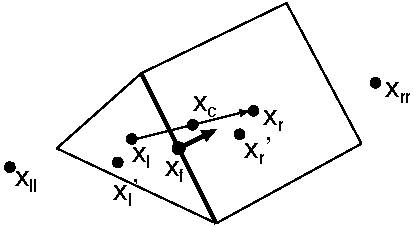
\includegraphics[width=0.5\textwidth]{flux_correct}
\caption{Geometry of flux stencil formation}
\label{fig:stencil}
\end{center}
\end{figure}


We can utilize the cell gradients computed on the left and right side
to devise a correction for the offset between $\vec{x}_f$ and
$\vec{x}_c$.  Note that the without this correction the scheme given
in Eq. (\ref{eq:fourth}) will degrade to first order on unstructured
grids unless mesh refinement is sufficiently smooth
(e.g. $|\vec{x}_f-\vec{x}_c| = O(h^2)$). A correction that will
restore second order accuracy for non-smooth refinements is
accomplished by using the cell centered gradients at the left and
right cells to shift the stencil such that it is centered on the face
center.  For a given interpolated value $\phi$, the states
interpolated to this new stencil are given by the correction
\begin{equation}
\begin{aligned}
{\phi_{l}}^{'} &= \phi_l + \nabla \phi_l \cdot (\vec{x}_f-\vec{x}_c)\\
{\phi_{r}}^{'} &= \phi_r + \nabla \phi_r \cdot (\vec{x}_f-\vec{x}_c),\\
\end{aligned}
\end{equation}
which provides a second order correction provided that $\nabla \phi$
is computed to at least first order accuracy.

To recover a $4^{th}$ order accurate scheme on Cartesian meshes we
need to establish a reconstruction for the left-of-left and
right-of-right stencil locations that will correspond to the actual
values at these cell locations on a Cartesian mesh, but are only
functions of the available left and right values and gradients.  To do
this we start with the assumption that gradients will be computed at
the cells using a least squares reconstruction.  For this
reconstruction on a Cartesian mesh, it can be show that the following
relationships will identically hold:
\begin{equation}
\begin{aligned}
\nabla \phi_l \cdot (\vec{x}_r-\vec{x}_l) = &\frac{\phi_{r}-\phi_{ll}}{2}\\
\nabla \phi_r \cdot (\vec{x}_r-\vec{x}_l) = &\frac{\phi_{rr}-\phi_{l}}{2}\\
\end{aligned}
\end{equation}

Using these relations, we can then compute an effective left-of-left
and right-of-right state using the cell values and their gradients.
These are defined as follows:
\begin{equation}
\begin{aligned}
{\phi_{ll}}^{'} &= {\phi_r}^{'} - 2 \nabla \phi_l \cdot (\vec{x}_r-\vec{x}_l) \\
{\phi_{rr}}^{'} &= {\phi_l}^{'} + 2 \nabla \phi_r \cdot (\vec{x}_r-\vec{x}_l) \\
\end{aligned}
\end{equation}

The approach produces exactly the $4^{th}$ order flux on Cartesian
grids and also provides a reasonable correction for general meshes.
This approach has the advantage of only requiring the cell centered
least squares gradient which will be required for the upwind flux as
was observed in a similar formulation presented by Darwish and
Moukalled\cite{Darwish.2003}.  Note, this implementation was arrived at
after evaluating many subtle variations on the themes presented here.
For example, a centered face interpolation using cubic polynomials is
evaluated to replace the face averaged values for the skew-symmetric
flux but did not produce $4^{th}$ order convergence on Cartesian
meshes due to the presence of aliased second order modes.  Similarly,
centered linear reconstructions at the face were evaluated to correct
for location of the face center, but the resulting scheme is less
stable and required more blended upwinding than the one presented
here.

\subsubsection{Hybrid Flux Scheme}

In practice the skew symmetric fluxes (equation (\ref{eq:fourth}))
fail for shocked flows and therefore need to be hybridized with standard
upwind fluxes to enable simulation of high speed flows.  In addition,
unstructured stencils can depart significantly from skew-symmetry and
thus will require some stabilizing dissipation which is provided by
blending to the upwind flux. This blending is achieved by using a
simple weighted average of central flux and upwind flux schemes such
that our final inviscid flux can be written as
\begin{equation}
F_i = (1-\alpha_{diss})F_{SSF} + \alpha_{diss} F_{upwind}.
\end{equation}
For this study we utilize the robust HLLC scheme\cite{Torro.1994} for
the upwind flux.  Since we are also using the upwind scheme to
stabilize corrections on unstructured meshes we modify the 
upwind scheme to provide low dissipation in low Mach number regions by
employing the simple scaling scheme proposed by Thornber {\it et
  al.}\cite{Thornber.2008} whereby the left and right velocity states
are modified according to the local face Mach number, $M_{f}$,
according to the relations:
\begin{equation}
\begin{aligned}
\vec{u}_{l,th} &= \frac{\vec{u}_l + \vec{u}_r}{2} + \min(M_{f},1) \frac{\vec{u}_l-\vec{u}_r}{2}\\
\vec{u}_{r,th} &= \frac{\vec{u}_l + \vec{u}_r}{2} + \min(M_{f},1) \frac{\vec{u}_r-\vec{u}_l}{2}\\
\end{aligned}
\end{equation}

Blending upwind fluxes will be motivated by three concerns: 1)
geometric concerns where upwinding is used to stabilize the central
flux schemes when skew-symmetry is lost, and 2) to provide a proper
amount of added dissipation in regions with dissipative structures
such as shocks and expansions, and 3) to provide a Monotone Implicit
LES model (MILES) approach to subgrid filtering by employing a small
amount of upwinding dissipation as an implicit subgrid model.
Therefore $\alpha_{diss}$ will be computed based on mesh geometry
($\alpha_{geom}$) and compressibility based ($\alpha_{comp}$), and
subgrid modeling based ($\alpha_{miles}$) considerations.  Ultimiately
$\alpha_{diss}$ will be determined by the maximum of these three
factors.  Since blending to upwinding generally introduces dissipation
to the scheme, we would like to keep the non-physics based
$\alpha_{geom}$ as small as possible.  We use a heuristic approach to
add dissipation based on angles formed by the face reconstruction
where each face blends to an upwind scheme independently.
Specifically we are concerned with two potentially problematic angles:
1) the angle between the face normal and the vector joining the cell
center should be as close to zero as possible, and 2) the angle of a
line that is tangent to a sphere centered on the skew-symmetric flux
center ($X_c$) with a radius containing the face centroid, $r_f =
|X_f-X_c|$ as illustrated in figure \ref{fig:stencilangle}.  The
geometric upwinding is computed based on the maximum of these two
angles, denoted as $\theta_{max}$.  Then the geometric based upwinding
is computed using the relation
\begin{equation}
\alpha_{geom} = \chi^2 + \frac{\eta_2}{\eta_1}*(\chi^3-2\chi^2+\chi); \chi
= \min\lbrace\eta_1(1-\cos~\theta_{max}),1\rbrace
\end{equation}
where $\eta_1$ selects the angle at which full upwinding will occur,
and $\eta_2$ controls how fast upwinding is added for small departures
from ideal mesh quality.  For the test cases studied it was found that
accurate and robust results were obtained with, $\eta_1=2$, which
provides full upwinding when $\theta_{max} = 60\deg$, while $\eta_2=1$
ensures stability on good quality meshes where small corrections are
applied keeping $\alpha_{geom} \sim 1-cos~\theta_{max}$ for small
angles.  In general, $\eta_1$ and $\eta_2$ are user adjustable
parameters, but the settings described here are effective for a wide
range of mesh configurations and appear to provide a reasonable
compromise between robustness and low dissipation.

\begin{figure}[h]
\begin{center}
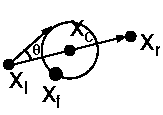
\includegraphics[width=0.5\textwidth]{geom_test}
\caption{Geometry of flux stencil formation}
\label{fig:stencilangle}
\end{center}
\end{figure}

Since the central flux scheme cannot properly resolve shocks, a method
must be used to identify regions of the flow that have shocks where it
is necessary to switch to an upwind scheme.  One of the more popular
shock detectors used for this purpose is the method originally
implemented by Ducros {\it et al.}\cite{Ducros.2000} which detects
shocks by comparing the magnitude of the divergence of velocity with
the vorticity.  Regions that are vorticity dominant (such as LES
regions) switch to the low dissipation flux.  However, this switch
often becomes active in regions where an upwind scheme is not
necessary.  In addition, refining a region of smooth flow will not
allow the code to switch to a lower dissipation flux.  Ideally a
switch should reduce the area where the upwind scheme is utilized with
mesh refinement, and so a switch that considers local mesh resolution
is desired.  This switch should be based on the magnitude of
divergence of the velocity field which gives a measure of the
rate of compression in the flow, a mesh length scale, and some measure of
the fluid response to compression, such as sound speed.  Using these
measures and dimensional analysis we arrive at the following
\begin{equation}
\alpha_{comp} = \left[\min\left(\eta_{comp}\frac{\left| \nabla \cdot
        \vec{u} \right| \delta x_{ref}}{a },1\right)\right]^2
\label{eq:alphacomp}
\end{equation}
where $a$ is the local sound speed, and $\delta x_{ref}$ is the cell
reference length defined as the diameter of the smallest sphere that
encloses all cell face centers.  The variable $\eta_{comp}$ is a user
defined sensitivity parameter.  The non-dimensional term is squared so
that the transition to the central scheme will correspond with mesh
refinement at a rate of $O(h^2)$ in smooth flow regions.  For the
studies that involve shocks presented here a value of $\eta_{comp} =
5$ is used.  Note, with this method the value for $\alpha_{comp}$ will
vanish with mesh refinement for any smooth solution, but will always
be active at shocks.  The final value for $\alpha_{diss}$ used by the
flux is defined by the maximum of the left and right values for
$\alpha_{comp}$ and the local face value for $\alpha_{geom}$.

%%\input{num_inviscid.tex}

%%\input{num_difftrans.tex}

\subsection{Time Integration}

For the time integration scheme we utilize a Crank-Nicholson inspired
scheme where the residual is evaluated an an interpolated half step.
The interpolated half step, denoted by the primitive variable vector
$q^{\star}$, is computed according to the relation
\begin{equation}
  q^{\star} = \left[ T^{\star}, \vec{u}^{\star}, p^{\star} \right ],
\label{half_step}
\end{equation}
where 
\begin{equation}
\begin{aligned}
  T^{\star} &= \frac{2 T^{n+1} ~ T^{n}}{T^{n+1} + T^{n}} \\
  \vec{u}^{\star} &= \frac{\sqrt{\rho^{n+1}} \vec{u}^{n+1}+\sqrt{\rho^{n}} \vec{u}^n} {\sqrt{\rho^{n+1}}+\sqrt{\rho^n}} \\
p^{\star} &= \frac{(1+\epsilon)p^{n+1} + (1-\epsilon)p^{n}}{2}\\
\label{eq:temporalavg}
\end{aligned}
\end{equation} 
This differs from the Subbareddy {\it et al.} \cite{Subbareddy.2009}
scheme in several important aspects.  First the average is defined in
terms of pressure and temperature to improve the performance
of the algorithm when there is a more complex EoS as mentioned
previously.  Second, a harmonic averaging of temperature is utilized
as this provides stability in high speed flow cases.  The energy
consistent form of velocity averaging is retained.  Note, the
$\epsilon$ pressure biasing in the pressure averaging is used to
provide the scheme with acoustic damping which is necessary when
running at high Courant-Friedrich-Lewy (CFL) numbers.  The effect of
this term will be elucidated in later discussions.  The time
integration can then be expressed as the solution to the non-linear
equation
\begin{equation}
\mathcal{L}(q^{\star})=\frac{\V}{\Delta t} (Q^{n+1} - Q^n) - R(q^{\star}) = 0 ,
\label{Lcn}
\end{equation}
where $Q = \left[ \rho, \rho\vec{u}, \rho e_T \right]$ is the
conservative variable vector where the total energy is $e_T =
e(p,T)+(\vec{u}\cdot \vec{u})/2$.  The residual, $R$, results from the
numerically integrated flux functions given by
\begin{equation}
R = \sum_{f=1}^{nf} \A_f \left( F_{v,f} - F_{i,f} \right)
\end{equation}
where $\A_f$ is the area of face $f$, and $F_v$ and $F_i$ are the
viscous and inviscid fluxes respectively.

The solution is advanced in time by solving eq. (\ref{Lcn}) by a
Newton iteration method which can be described as follows
\begin{equation}
\mathcal{L}'(q^{\star, n+1,k}) (q^{\star,n+1,k+1} - q^{\star, n+1,k}) = -\mathcal{L}
(q^{\star,n+1,k}), \label{new}
\end{equation}
for $k\geq 0$, where the Newton iteration is initialized using the
previous time step value ($q^{\star,n+1,k=0} = q^{\star,n}$). To limit
the size of the jacobian of operator $\mathcal{L}$, only the first
order parts of the flux stencils are retained.  For the inviscid flux
jacobians we utilize approximate jacobians of the HLLC flux as
described by Batten {\it et al.} \cite{Batten.2006} even when the
skew-symmetric fluxes are utilized. These jacobian approximation
errors have no effect on the solution once the Newton method is
converged.


\subsubsection{Local Time-Stepping Scheme}

When running in steady timestepping mode the code utilizes a local
timestep based on estimated changes in local pressure and temperature.
This estimate is base on a first order explicit step whereby the
estimated rate of change in pressure and temperature can be determined
through solving the inverse of the jacobian of the conservative
variables with respect to the primitive variables times the source
terms formed from the invisicd and viscous fluxes.  The timestep that
will limit the change of these variables no more than the
$\mu_{relax}$ factor is computed from these rates.  If this timestep
is smaller than the specified maximum timestep, then the smaller value
will be used.


%%\subsection{Jacobian Formulations}

The Jacobian matrix used in the Newton method, described by
Eq.~(\ref{Jacobian}), consists of a block-diagonal matrix, formed from
Jacobians of chemistry source terms, combined with both diagonal and
off-diagonal matrices, formed from the differentiation of flux functions.
When constructing this Jacobian, one takes advantage of the fact that
the flux function, $\hat{F}(q_{l}, q_{r})$,
is defined by the conservative variables on the left and
right side of the face.  Then the Jacobian of this function will
consist of two matrices, given by
\begin{equation}
\begin{split}
fjl & = \mathcal{A}^{n+1}\frac{\partial \hat{F}(q_{l},q_{r})}{\partial q_{l}},\\
fjr & = \mathcal{A}^{n+1}\frac{\partial \hat{F}(q_{l},q_{r})}{\partial q_{r}}.
\end{split}
\end{equation}
The variables above, {\tt fjl} and {\tt fjr}, are Jacobians of the flux
functions located at faces and are components of the overall Jacobian
matrix given in Eq.~(\ref{Jacobian}).
More details on the final form of the Jacobian matrix are given by 
Luke\cite{luke.99}.

\subsubsection{Inviscid Flux Jacobians}

In the study, all Jacobians are evaluated analytically, except for the
inviscid flux, whereby Jacobians associated with the Roe scheme are
too complex to implement efficiently.  In this case, several
alternatives are available: 1) use analytic Jacobians of simpler
inviscid flux functions such as Steger-Warming or Van Leer, or 2)
compute Jacobians of the Roe flux numerically. The
analytic Van Leer Jacobian was found to provide superior stability properties,
but severely hampered convergence of the implicit scheme.  On the
other hand, the numerical Roe Jacobians provided better convergence
rates, but sometimes produced ill-conditioned linear systems.  It was
observed that these problems occurred in regions where discontinuities
existed in the Roe Jacobians, due to the use of non-linear absolute
value functions.  A compromise that appears to provide a reasonable
balance between convergence and robustness has been found by smoothing
the Roe flux function before taking its derivative.  This is
accomplished by replacing the absolute value function $|x|$ with the continuous
function $\sqrt{x^2+\epsilon}$, where $\epsilon$ is set to $.05$ times
the average sound speed.

\subsubsection{Viscous Flux Jacobians}

In the construction of viscous flux Jacobians, a thin-layer
approximation is used in the representation of the face gradient by
using simple centered differences in the direction of the vector
connecting cell centroids on either side of the face.

\subsubsection{Jacobians for Turbulence Models}

In order to preserve the diagonal dominance of the matrix in the
linear system, positive parts of the source terms are not linearized:
only the negative parts (which model the destruction of turbulence)
are included in the Jacobians.  For the Jacobians used in the BSL,
SST, and $k-\omega$ models the approach of Merci {\sl et
  al.\/}\cite{Merci.00} is adopted.



%%\subsection{Scalar Transport Equations}

The scalar transport equation in conservative form is written for a
convected scalar, $\phi$ as
\begin{equation}
\frac{\partial \rho \phi}{\partial t} + \nabla \cdot (\rho u \phi) = \nabla\cdot(\lambda \nabla \phi) + S_\phi,
\end{equation}
where $\rho$ is the fluid density, $u$ is the fluid velocity vector,
$\lambda$ is a diffusion coefficient, and $S_\phi$ is a prescribed
source term.  We note that by substituting $\phi=1$ into the above
equation one recovers the global continuity equation.  We discretize
the above equation in time and space to arrive at the expression
\begin{eqnarray}
\frac{\V}{\Delta t} \left[ (1+\psi)(\phi^{n+1}\rho^{n+1}-\phi^n\rho^n) + \psi(\phi^n\rho^n-\phi^{n-1}\rho^{n-1})\right ] = \\\nonumber
 -\sum\phi^{n+1}_u\dot{m}_f + \sum{D_\phi}_f + S_\phi,
\label{eq:scalar1}
\end{eqnarray}
where $\phi_u$ is an upwinded extrapolation of $\phi$ based on the
sign of the face mass flux $\dot{m}$ and ${D_\phi}_f$ is the numerical
diffusion flux for scalar $\phi$.  Note that the discrete continuity equation is given by
\begin{equation}
\frac{\V}{\Delta t} \left[ (1+\psi)(\rho^{n+1}-\rho^n) + \psi(\rho^n-\rho^{n-1})\right ] = - \sum\dot{m}_f.
\label{eq:continuityN}
\end{equation}

To improve the diagonal dominance of the scheme we employ a trick
where we recognize that Eq. (\ref{eq:continuityN}) is zero when
the system of equation is solved, thus we multiply Eq.
(\ref{eq:continuityN}) by $\phi^{n+1}$ and subtract it from Eq.
(\ref{eq:scalar1}) to arrive at the following expression:
\begin{eqnarray}
\frac{\V}{\Delta t} \left[ \left(1+\psi\right)\left(\phi^{n+1}-\phi^n\right)\rho^n + \left(\phi^n\rho^n-\phi^{n-1}\rho^{n-1}\right)\psi-\left(\rho^n-\rho^{n-1}\right)\phi^{n+1}\psi\right ] - \\\nonumber
\left[\phi^{n+1}\sum\dot{m}_f-\sum\phi^{n+1}_u\dot{m}_f + \sum{D_\phi}_f + S_\phi\right] =L_\phi(\phi^{n+1}) = 0.
\label{eq:scalar2}
\end{eqnarray}
The above operator, $L_\phi$, is solved using a Newton method concurrently with the fluid equations.




\bibliography{guide}
\bibliographystyle{unsrt}

\end{document}




